% Paquets généraux
\documentclass[a4paper,12pt,titlepage,twoside]{article}
\usepackage[T1]{fontenc}
\usepackage[utf8]{inputenc}
\usepackage[french]{babel}
\usepackage{subcaption}
\addto\captionsfrench{%
  \renewcommand{\tablename}{Tableau}%
}
\usepackage[gen]{eurosym}
%\usepackage[dvips]{graphicx}
\usepackage{minted}
\usepackage{fancyhdr}
\usepackage{pdfpages} 
\usepackage{multido}
\usepackage{hyperref}
\usepackage{textcomp}
\usepackage{schemabloc}
%\usepackage[bitstream-charter]{mathdesign}
\usepackage{array}
\newcolumntype{P}[1]{>{\centering\arraybackslash}p{#1}}
\usepackage[shortlabels]{enumitem}
\usepackage[framemethod=TikZ]{mdframed}

\newcommand{\id}{71}
\newcommand{\nom}{Théorie des mécanismes}
\newcommand{\sequence}{04}
\newcommand{\nomsequence}{Liaisons entre les solides}
\newcommand{\num}{02}
\newcommand{\type}{KH}
\newcommand{\descrip}{Liaisons équivalentes, hyperstatisme, liaisons en série et en parallèle, théorie des graphes}
\newcommand{\competences}{B2-12: Proposer une modélisation des liaisons avec leurs caractéristiques géométriques. \\ &  B2-13: Proposer un modèle cinématique paramétré à partir d'un système réel, d'une maquette numérique ou d'u \\ &  B2-17: Simplifier un modèle de mécanisme. \\ &  B2-18: Modifier un modèle pour le rendre isostatique. \\ &  C1-04: Proposer une démarche permettant d'obtenir une loi entrée-sortie géométrique.  \\ &  C2-05: Caractériser le mouvement d'un repère par rapport à un autre repère. \\ &  C2-06: Déterminer les relations entre les grandeurs géométriques ou cinématiques. }
\newcommand{\nbcomp}{7}
\newcommand{\systemes}{}
\newcommand{\systemesnum}{}
\newcommand{\systemessansaccent}{}
\newcommand{\ilot}{2}
\newcommand{\ilotstr}{02}
\newcommand{\dossierilot}{\detokenize{Ilot_02 }}

%\usepackage{style}
\usepackage{bodegraph}
\usepackage{rpcinematik}
\usepackage[locale = FR]{siunitx}
\usepackage{caption}
\newcommand{\institute}{Lycée Dorian}

\usepackage{listings}
\usepackage{fancyvrb}
\usepackage{color}
\usepackage{xcolor}
\usepackage{colortbl}
\usepackage{helvet}
\usepackage[frenchmath]{newtxsf} % for sans serif symbols
\renewcommand{\familydefault}{\sfdefault}
%\usepackage{amsfonts}
%\usepackage{amsmath}
%\usepackage{lmodern}
\usepackage{mathastext}
%\usepackage{xspace}
\usepackage{varioref}
\usepackage{tabularx}
%\usepackage{floatflt}
\usepackage{graphics}
\usepackage{wrapfig}
\usepackage{textcomp}
\usepackage{tikz,tkz-tab}
\usepackage[european resistor, european voltage, european current]{circuitikz}
\usepackage{wrapfig}
\usepackage{gensymb}
\usepackage[percent]{overpic}
\usetikzlibrary{babel}
\usepackage{ifthen}
\usepackage{cancel}
\usepackage{etoolbox}
\usepackage{multirow}
%\usepackage{boxedminipage}
\definecolor{gris25}{gray}{0.75}
\definecolor{bleu}{RGB}{18,33,98}
\definecolor{bleuf}{RGB}{42,94,171}
\definecolor{bleuc}{RGB}{231,239,247}
\definecolor{bleum}{RGB}{160,195,226}
\definecolor{rougef}{RGB}{185,18,27}
\definecolor{rougec}{RGB}{255,188,204}%255,230,231
\definecolor{vertf}{RGB}{103,126,82}
\definecolor{vertc}{RGB}{220,255,191}
\definecolor{forestgreen}{rgb}{0.13,0.54,0.13}
\definecolor{blcr}{rgb}{0.59,0.69,0.84}
\definecolor{blfr}{rgb}{0.32,0.51,0.75}
\definecolor{orfr}{rgb}{0.90,0.42,0.15}
\definecolor{orcr}{rgb}{0.90,0.65,0.50}
\definecolor{orangef}{rgb}{0.659,0.269,0.072}
\definecolor{orange}{rgb}{0.58,0.35,0.063}
\definecolor{orangec}{rgb}{0.43,0.32,0.25}
\definecolor{rcorrect}{rgb}{0.6,0,0}
\definecolor{sequence}{rgb}{0.75,0.75,0.75}
\definecolor{competences}{rgb}{0.61,0.73,0.35}
\definecolor{rose}{HTML}{ff00ff}
\definecolor{grisf}{HTML}{222222}
\definecolor{grisc}{HTML}{636363}
\definecolor{normal}{HTML}{4087c4}
\definecolor{info}{HTML}{5bc0de}
\definecolor{success}{RGB}{92,184,92}
\definecolor{warning}{RGB}{240,173,78}
\definecolor{danger}{RGB}{217,83,79}
\hypersetup{                    % parametrage des hyperliens
    colorlinks=true,                % colorise les liens
    breaklinks=true,                % permet les retours à la ligne pour les liens trop longs
    urlcolor= blfr,                 % couleur des hyperliens
    linkcolor= orange,                % couleur des liens internes aux documents (index, figures, tableaux, equations,...)
    citecolor= forestgreen                % couleur des liens vers les references bibliographiques
    }

\newcolumntype{M}[1]{>{\centering\arraybackslash}m{#1}}
\definecolor{codegreen}{rgb}{0,0.6,0}
\definecolor{codegray}{rgb}{0.5,0.5,0.5}
\definecolor{codepurple}{rgb}{0.58,0,0.82}
\definecolor{backcolour}{rgb}{0.95,0.95,0.92}

\lstdefinestyle{mystyle}{
    backgroundcolor=\color{backcolour},   
    commentstyle=\color{codegreen},
    keywordstyle=\color{magenta},
    numberstyle=\tiny\color{codegray},
    stringstyle=\color{codepurple},
    basicstyle=\ttfamily\footnotesize,
    breakatwhitespace=false,         
    breaklines=true,                 
    captionpos=b,                    
    keepspaces=true,                 
    numbers=left,                    
    numbersep=5pt,                  
    showspaces=false,                
    showstringspaces=false,
    showtabs=false,                  
    tabsize=2
}

\lstset{style=mystyle}

% Mise en page
\pagestyle{fancy}

\setlength{\hoffset}{-18pt}
\setlength{\oddsidemargin}{0pt} 	% Marge gauche sur pages impaire2s
\setlength{\evensidemargin}{0pt} 	% Marge gauche sur pages paires
\setlength{\marginparwidth}{00pt} 	% Largeur de note dans la marge
\setlength{\headwidth}{481pt} 	 	% Largeur de la zone de tête (17cm)
\setlength{\textwidth}{481pt} 	 	% Largeu\textbf{r de la zone de texte (17cm)
\setlength{\voffset}{-18pt} 		% Bon pour DOS
\setlength{\marginparsep}{7pt}	 	% Séparation de la marge
\setlength{\topmargin}{-30pt} 		% Pas de marge en haut
\setlength{\headheight}{55pt} 		% Haut de page
\setlength{\headsep}{20pt} 		% Entre le haut de page et le texte
\setlength{\footskip}{30pt} 		% Bas de\textbf{ page + séparation
\setlength{\textheight}{700pt} 		% Hauteur de l'icone zone de texte (25cm)
\setlength\fboxrule{1 pt}
\renewcommand{\baselinestretch}{1}
\setcounter{tocdepth}{1}
\newcommand{\cadre}[2]
{\fbox{
  \begin{minipage}{#1\linewidth}
   \begin{center}
    #2\\
   \end{center}
  \end{minipage}
 }
}

\newcommand{\repon}[1]
{
~\ \\
\begin{tabular}{|m{\linewidth}|}
 \hline
\multido{}{#1}{\\ \hline}
\end{tabular}
}


\newcommand{\objectif}[1]{
\mdfsetup{%
frametitle={%
\tikz[baseline=(current bounding box.east),outer sep=0pt]
\node[anchor=east,rectangle,fill=bleum]
{\strut Objectif~};}}
\mdfsetup{innertopmargin=10pt,linecolor=bleum,%
linewidth=2pt,topline=true,%
frametitleaboveskip=\dimexpr-\ht\strutbox\relax
}
\begin{mdframed}[]\relax%
#1
\end{mdframed}}


\newcounter{num_quest} \setcounter{num_quest}{0}
\newcounter{num_rep} \setcounter{num_rep}{0}
\newcounter{num_cor} \setcounter{num_cor}{0}

\newcommand{\feuilleDR}[1]{
	\begin{tikzpicture}
		\draw[gray!30](0,0)grid[step=0.5cm](\linewidth,#1);
	\end{tikzpicture}
}

%\newcommand{\question}[1]{\refstepcounter{num_quest}\par
%~\ \\ \parbox[t][][t]{0.15\linewidth}{\textbf{Question \arabic{num_quest}}}\parbox[t][][t]{0.85\linewidth}{#1\label{q\the\value{num_quest}}}\par
%}

\newcommand{\question}[1]{\refstepcounter{num_quest}\par
~\ \\ \textbf{Question \arabic{num_quest} : }#1\label{q\the\value{num_quest}}\par
}

\newcommand{\posetafigure}[3]{
\begin{figure}[ht!]
 \begin{center}
  \includegraphics[width=#2\linewidth]{img/#1}
 \end{center}
 \caption{\label{#1} #3}
\end{figure}}

\newcommand{\goforum}{
\begin{figure}

\end{figure}
\begin{center}
 
\includegraphics[width=0.7\linewidth]{../../../img/go_forum}
\end{center}
\label{go_forum}
\caption{J'pète les plombs}
\end{figure}}

\newcommand{\reponse}[4][1]
{\noindent
\parbox{\textwidth}{
\rule{\linewidth}{.5pt}\\
\textbf{Question\ifthenelse{#1>1}{s}{} \multido{}{#1}{%
\refstepcounter{num_rep}\ref{q\the\value{num_rep}} }:} ~\ \\
\ifdef{\public}{#3 \ifthenelse{#2>0}{~\ \\ 	\feuilleDR{#2}}}{#4}
}}

\newcommand{\cor}
{\refstepcounter{num_cor}
\noindent
\rule{\linewidth}{.5pt}
\textbf{Question \arabic{num_cor}:} \\
}

\newcommand{\finsujet}
{
    \begin{center}
    \Large{FIN}
    \end{center}

    \cleardoublepage

    \ifdef{\public}{\pagestyle{docreponse}}{\pagestyle{correction}}

    \ifdef{\public}{
        \begin{tikzpicture} 
            \draw (0,0) rectangle (2,2);
            \draw (0,0) -- (2,2);
            \draw (1.5,0.5) node {\large 20};
            \draw (2.5,0) rectangle (16,2);
            \draw (4.5,1.7) node {\large Commentaires:};
        \end{tikzpicture}
    }
    ~\ \\
}


%\newcommand{\repcarre}[2]
%{
%~\ \\
%\begin{tikzpicture}
%\draw [fill=white] (0,0) rectangle +(\linewidth,#1);
%\node[align=left] at (1.1,#2-0.3) {\textbf{Question #1:}};
%\end{tikzpicture}
%}

\newcommand{\titre}[1]
{\begin{center}
\cadre{0.8}{\huge #1} 
\end{center}
}


%Définition des torseurs :
\newcommand{\torseur}[2]{\left\{\mathcal{#1}_{#2} \right\}}
\newcommand{\torseurh}[3]{\left\{\genfrac{}{}{0pt}{0}{#1}{#2}\right\}_{#3}}
\newcommand{\torseurv}[8]{\left\{
\begin{matrix}
#1 & #4 \\ #2 & #5 \\ #3 &#6
\end{matrix}
\right\}_{{#7},{#8}}}

%Définition des torseurs :
%\newcommand{\torseur}[2]{\left \{\mbox{\relsize{2}{$\mathcal {#1}$}\relsize{-2}}\phantom{}_{\mbox{\scriptsize $#2$}} \right \}}
%\newcommand{\torseurh}[3]{\left\{\genfrac{}{}{0pt}{0}{#1}{#2}\right\}_{#3}}
%\newcommand{\torseurv}[8]{
%\left\{\begin{array}{@{}c|c@{}} #1 & #4 \\ #2 & #5 \\ #3 & #6 \end{array} \right\}_{#7,#8}
%}
\newcommand{\derivee}[2]{\left.\dfrac{\d #1}{\d t}\right|_{#2}}
\newcommand{\tripleint}{\int\!\!\!\!\!\int\!\!\!\!\!\int}

% Notation cinématique et statique
\newcommand{\cinematique}[2]{\mbox{#1}/\mbox{#2}}
\newcommand{\statique}[2]{\mbox{#1}\rightarrow\mbox{#2}}
\newcommand{\moment}[3]{\vv {#1}_{\scriptsize{#3}}(#2)}
\newcommand{\resultante}[2]{\vv {#1}_{\scriptsize{#2}}}


%Commande de base
\newcommand{\jo}{\left(j\omega\right)} % j \omega dans l'analyse fréquentielle
\newcommand{\tl}{\xrightarrow{\mathcal{L}}} % transformée de laplace sur fleche
\newcommand{\tli}{\xrightarrow{\mathcal{L}^{-1}}} % transformée inverse de laplace sur fleche
\renewcommand{\d}[1][]{\mathrm{d#1}}
\newcommand{\dd}[1][]{\mathrm{d#1}}
\newcommand{\vect}[2]{{#1}\wedge{#2}}
\newcommand{\base}[3]{(\vec #1,\vec #2,\vec #3)}
\newcommand{\vectbase}[4]{{\vphantom{\left| \begin{matrix}
#1\\#2\\#3 \end{matrix} \right|}}_{#4}{\left| \begin{matrix}
#1\\#2\\#3 \end{matrix} \right.}}
%Pour avoir les paragraphes sous la forme I, II, III
\renewcommand{\thesection}{\Roman{section}}
\setcounter{secnumdepth}{3}
\renewcommand{\Frlabelitemii}{$\bullet$}

% En tête et pied de page
\lhead{\nom}
\rhead{
\includegraphics[width=2cm]{../../../img/logo}}
\lfoot{\auteurun,\ \auteurdeux}
\cfoot{Page \thepage}

\fancypagestyle{docreponse}{%
  \fancyhf{}
  \fancyhead[LO]{NOM Prénom: .............................}
  \rhead{
\includegraphics[width=2cm]{../../../img/logo}\hspace{2pt}}
  \ifdef{\auteurdeux}{\lfoot{\auteurun,\ \auteurdeux}}{\lfoot{\auteurun}}
  \rfoot{\nom}
  \lfoot{Document réponse}
  \cfoot{Page \thepage}
   }

\fancypagestyle{correction}{%
  \fancyhf{}
  \lhead{\colorbox{danger}{\begin{minipage}{0.65\paperwidth} \textcolor{white}{\textbf{Correction}} \end{minipage}} }
  \rhead{
\includegraphics[width=2cm]{../../../img/logo}}
  \lfoot{Renaud Costadoat, Françoise Puig}
  \rfoot{\colorbox{danger}{\begin{minipage}{0.4\paperwidth} \begin{flushright}\textcolor{white}{\textbf{Correction}}\end{flushright} \end{minipage}} }}

\fancypagestyle{correctioninfo}{%
  \fancyhf{}
  \lhead{\colorbox{danger}{\begin{minipage}{0.65\paperwidth} \textcolor{white}{\textbf{Correction}} \end{minipage}} }
  \rhead{
\includegraphics[width=2cm]{../../../img/logo}}
  \lfoot{Renaud Costadoat, Juliette Genzmer}
  \rfoot{\colorbox{danger}{\begin{minipage}{0.6\paperwidth} \begin{flushright}\textcolor{white}{\textbf{Correction}}\end{flushright} \end{minipage}} }}

\renewcommand{\footrulewidth}{0.4pt}

\usepackage{eso-pic}
\newcommand{\BackgroundPic}{%
\put(0,0){%
\parbox[b][\paperheight]{\paperwidth}{%
\vfill
\begin{center}
\hspace{0.5cm}\vspace{0.5cm}

\includegraphics[width=\paperwidth,height=\paperheight,%
keepaspectratio]{../../../img/fond3}%
\end{center}
\vfill
}}}

\newcommand{\BackgroundPicdeux}{%
\put(25,-30){%
\parbox[b][\paperheight]{\paperwidth}{%
\vfill
\begin{center}
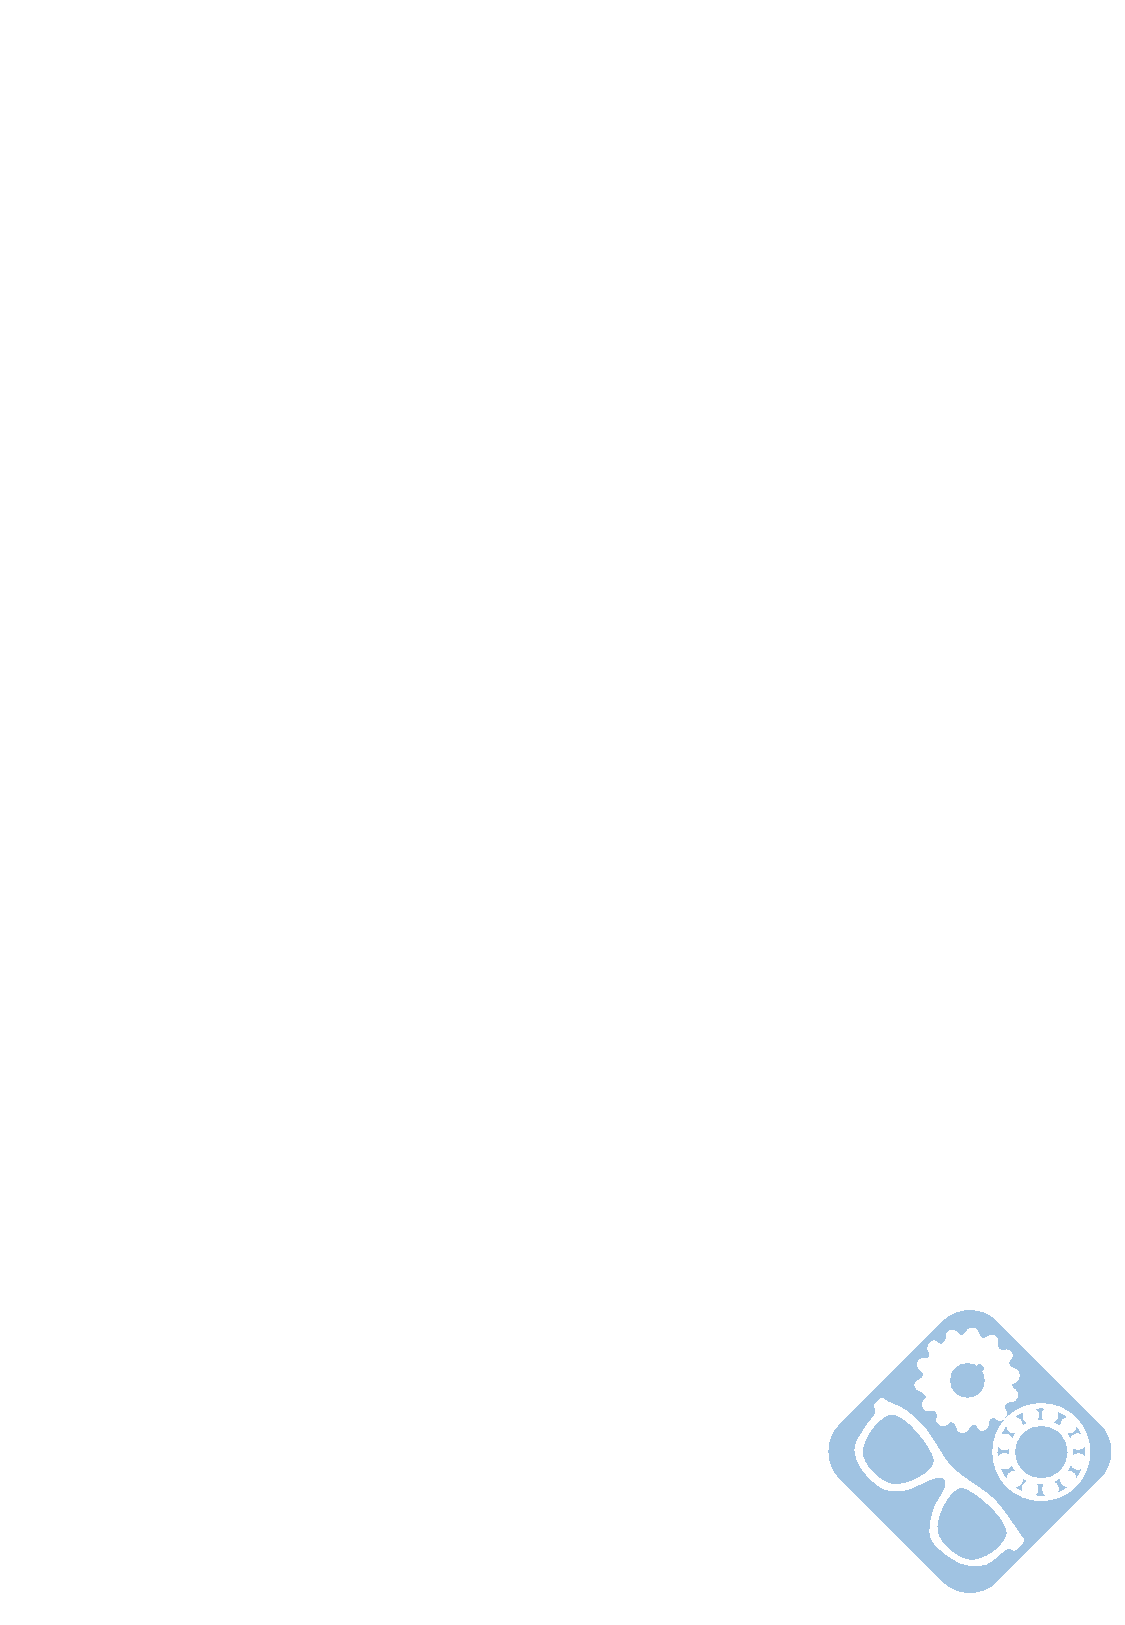
\includegraphics[width=\paperwidth,height=\paperheight,%
keepaspectratio]{../../../img/fond4}%
\end{center}
\vfill
}}}

\begin{document}

\pagestyle{empty}

\AddToShipoutPicture*{\BackgroundPic}


\includegraphics[width=2cm]{../../../img/logo}

\Huge{DS \numero - \sujet}

\vspace{1cm}

\ifdef{\prive}{\begin{center}\colorbox{danger}{\Huge{Avec Correction}}\end{center}}{}

\begin{center}
\centering\huge{PTSI}
\end{center}

\vspace{2cm}


\begin{center}
\centering\Large{\jour}
\end{center}

\vspace{2cm}

\normalsize

\tableofcontents

\newpage

\AddToShipoutPicture{\BackgroundPicdeux}

\pagestyle{fancy}

\begin{center}
\Huge \sujet
\end{center}


\normalsize


\section{Présentation}

\begin{figure}[ht!]
\begin{center}
 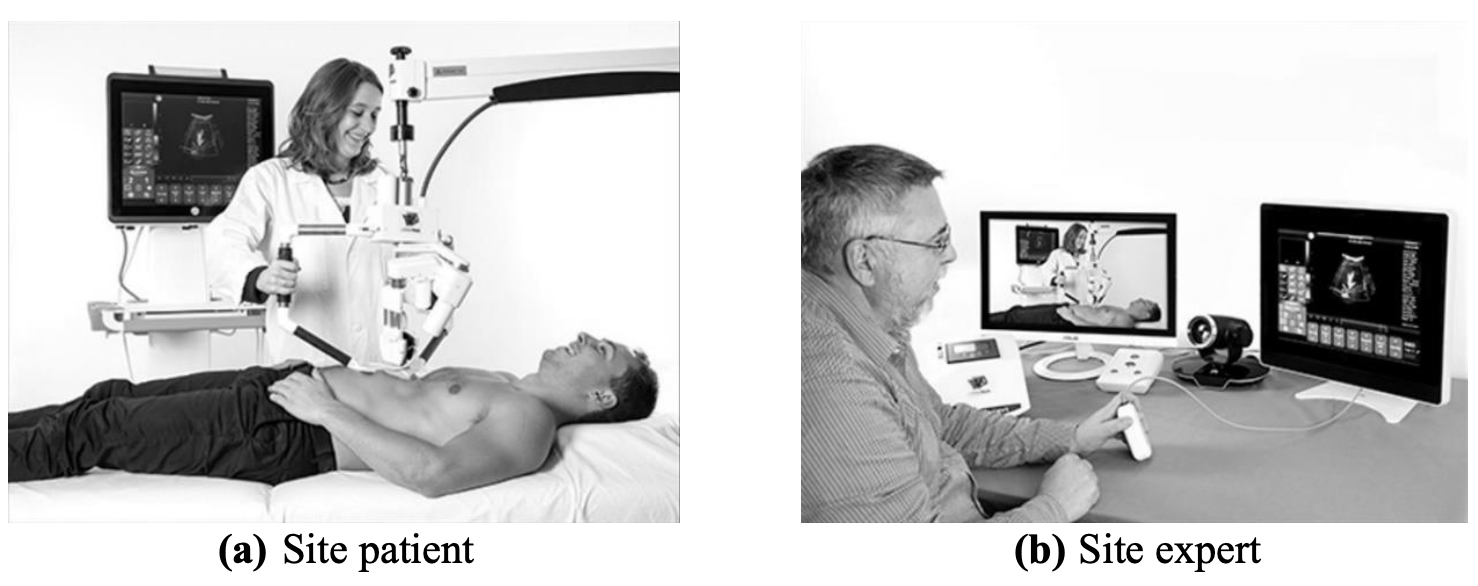
\includegraphics[width=0.9\linewidth]{img/fig01}
\end{center}
\caption{Principe de la télé-échographie}
\label{fig01}
\end{figure}

\subsection{Mise en situation}

L’échographie est une technique d’imagerie médicale basée sur l’exploitation de la réflexion d’une onde ultrasonore au niveau des interfaces physiologiques entre organes. Non irradiante, peu coûteuse et mobile, elle représente l’examen d’imagerie médicale le plus pratiqué au monde. En contrepartie, sa réalisation nécessite un manipulateur expert en imagerie médicale, capable d’analyser les images échographiques en temps réel afin d’orienter la sonde en conséquence. 

L’analyse et l’expertise sont donc réalisées pendant l’examen. De ce fait, cette technique d’imagerie est qualifiée de \og manipulateur dépendant \fg : sa mise en \oe uvre est difficilement envisageable sur des sites isolés. 

La robotisation de cette technique permet toutefois d'en élargir le champ d'application. Grâce à la télé-échographie robotisée (figure \ref{fig01}), il devient possible de réaliser une échographie sur un patient situé sur un site isolé (appelé site patient), alors même que le spécialiste en imagerie médicale se trouve sur un site distant de celui où est pratiqué l'examen (appelé site expert). 

Sur le site patient (figure \ref{fig01}-a) équipé du robot porte-sonde, d'un échographe et d'un système de visioconférence, un professionnel de santé est chargé de positionner le robot porte-sonde sur le patient et de le maintenir au cours de l'examen. Depuis le site expert distant (figure \ref{fig01}-b), le médecin dirige l'examen échographique. En manipulant une sonde fictive, il donne une consigne de position pour la sonde, que le robot exécute au contact du patient. Réalisant le lien entre les deux sites, le réseau de communication (ISDN, 4G, satellite...) permet en temps réel, le contrôle du robot, la visioconférence ainsi que la transmission des images échographiques. 

\subsection{Analyse système partielle}

Le diagramme d'exigences donné en Annexe, présente un extrait du cahier des charges du système de télé-échographie. 

La figure \ref{fig02} décrit le robot porte-sonde constitué :
\begin{itemize}
 \item d'une structure porteuse 0;
 \item d'un module de rotation, composé des sous-ensembles 1, 2, 3 permettant d'orienter la sonde en lui imposant trois rotations ($R_1$, $R_2$, $R_3$) suivant les axes 1 à 3 ;
 \item du porte-sonde 4 sur lequel est fixé la sonde échographique S. La translation T suivant l'axe 4 permet de contrôler l'effort de contact sonde/peau du patient.
\end{itemize}

\begin{figure}[ht!]
\begin{minipage}{0.45\linewidth}
\begin{center}
 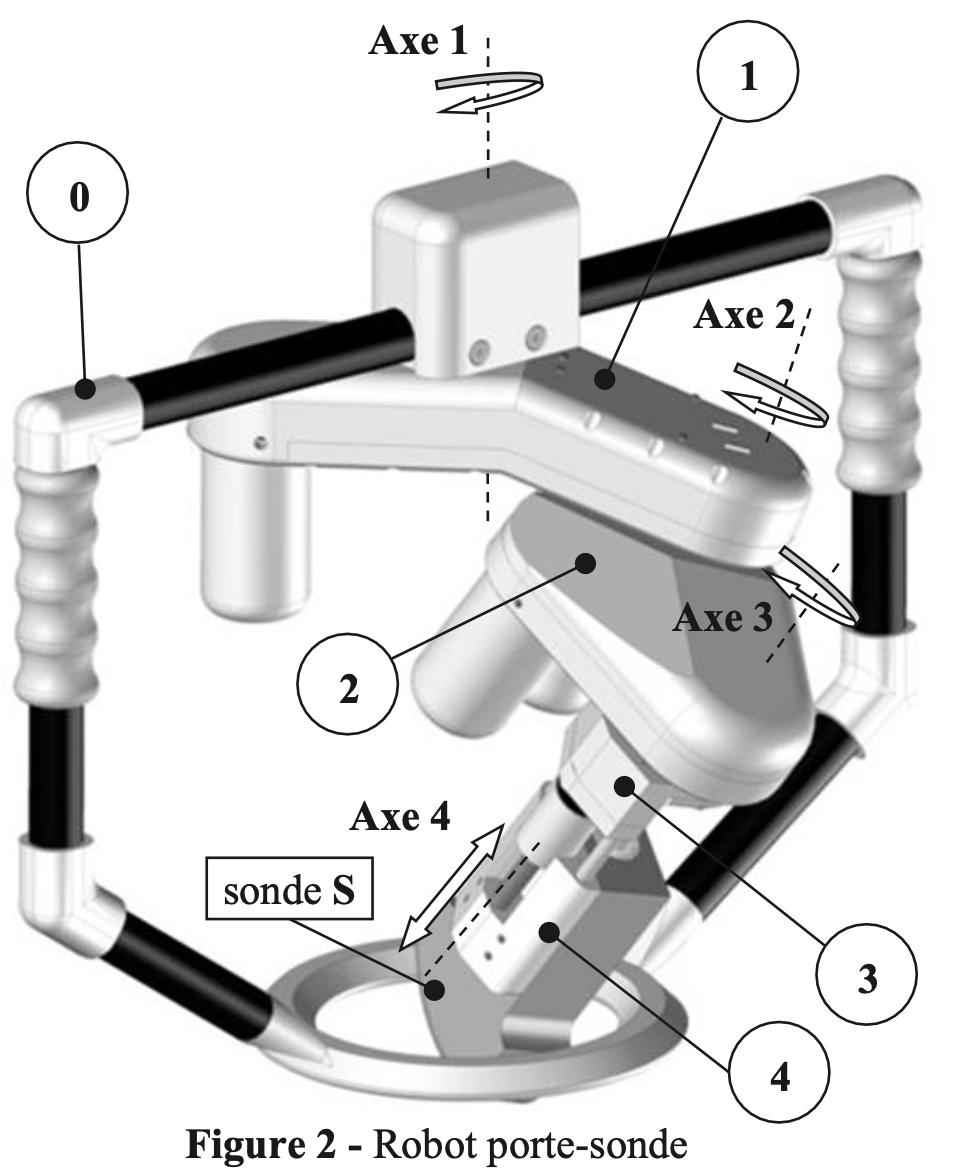
\includegraphics[width=0.9\linewidth]{img/fig02}
\end{center}
\caption{Robot porte-sonde}
\label{fig02}
\end{minipage}\hfill
\begin{minipage}{0.45\linewidth}
\begin{center}
 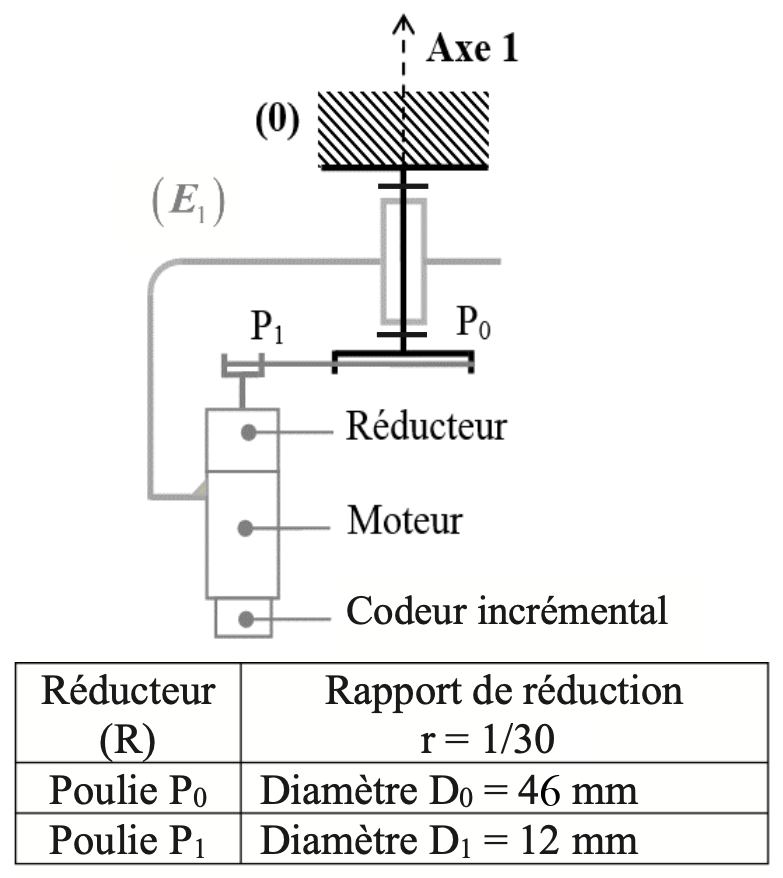
\includegraphics[width=0.9\linewidth]{img/fig03}
\end{center}
\caption{Caractéristiques de la transmission}
\label{fig03}
\end{minipage}
\end{figure}

On nomme $E_1$ l'ensemble ${1, 2, 3, 4}$.

\begin{figure}[ht!]
\begin{center}
 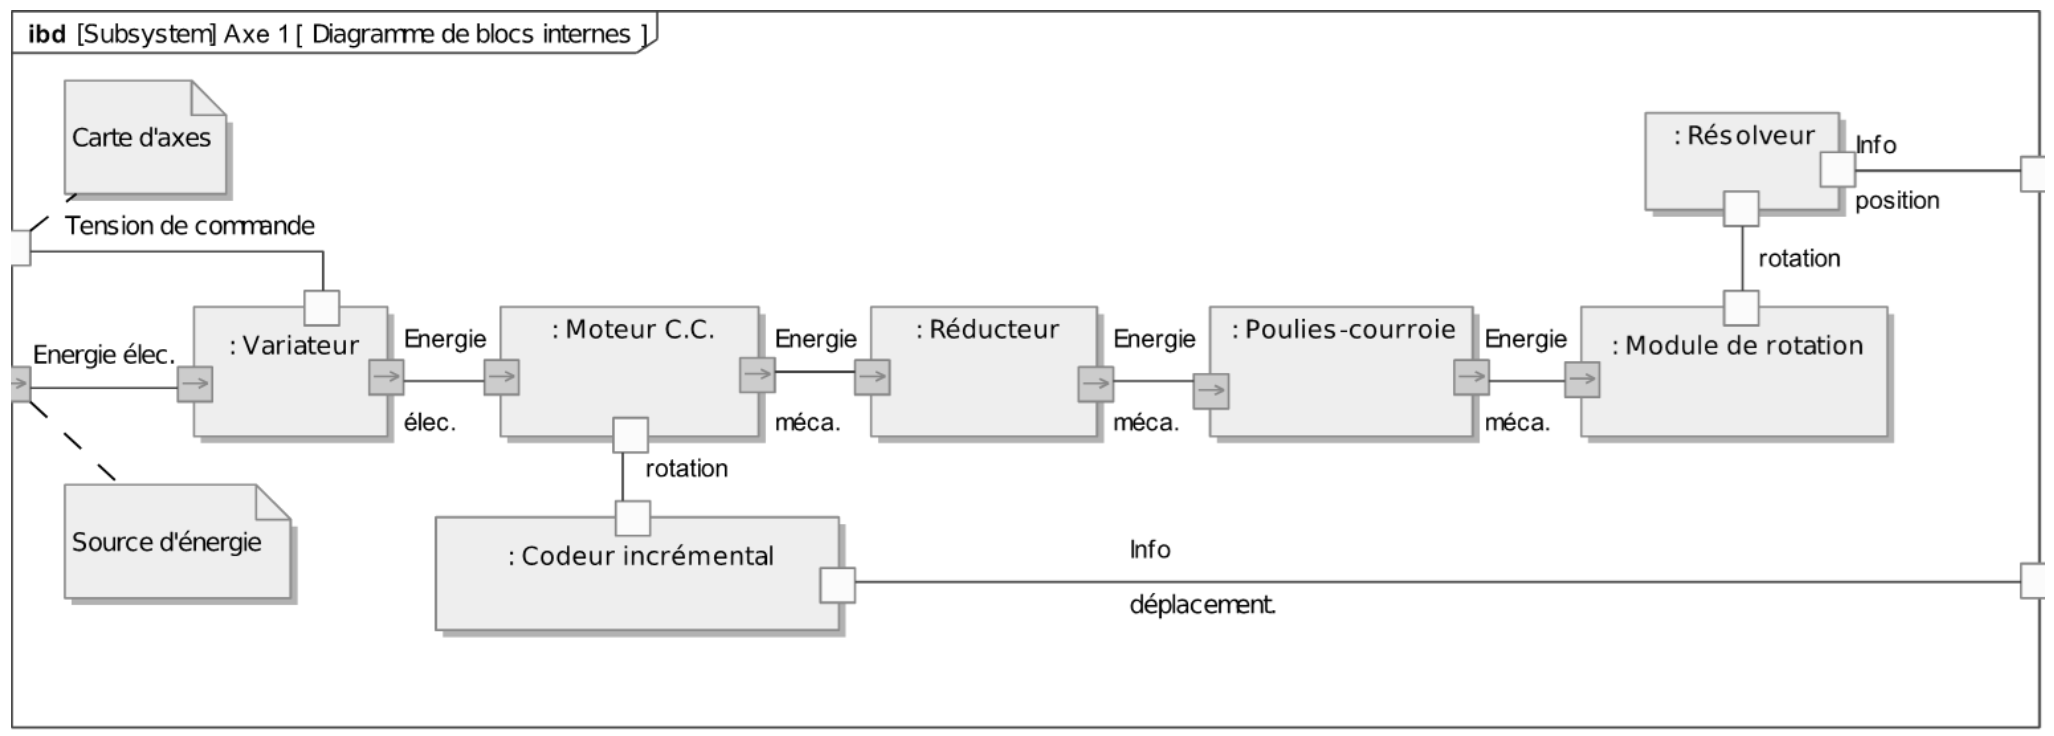
\includegraphics[width=0.9\linewidth]{img/fig04}
\end{center}
\caption{Diagramme de blocs internes de l'axe 1}
\label{fig04}
\end{figure}

La chaîne fonctionnelle assurant la rotation $R_1$ de l'ensemble $E_1$ autour de l'axe 1 est décrite par le schéma cinématique de la figure \ref{fig03} et le diagramme de bloc internes de la figure \ref{fig04}.

\subsection{Problème posé}

Afin que le praticien soit en mesure d'obtenir une image échographique d'intérêt, le système de télé- échographie doit lui permettre d'orienter la sonde de manière à trouver la meilleure incidence entre le plan ultrasonore et la partie de l'organe examinée. La qualité du positionnement de la sonde sur le patient qui conditionne l'obtention d'images d'intérêt nécessite de maîtriser notamment : 
\begin{itemize}
 \item le mouvement imposé à la sonde par le robot porte-sonde ;
 \item la commande, depuis un site distant, des différents axes du robot porte-sonde.
\end{itemize}

L'objectif de cette étude est de vérifier certaines performances du système afin de valider partiellement le respect des exigences liées au positionnement de la sonde échographique. 

\subsection{Démarche proposée}

Le respect des exigences 1.1 relatives au déplacement de la sonde fait l'objet de la Partie 2. Celle-ci a pour objectif de vérifier que la structure mécanique retenue est compatible avec les exigences liées au mouvement à imposer à la sonde (exigence 1.1.1) et à l'espace de travail attendu (exigence 1.1.2).

Le respect des exigences 1.2 relatives à la commande du robot porte-sonde est abordé à travers les points suivants prévision des performances et synthèse de la commande du premier axe du robot, en vitesse (exigence 1.2.1.1) et en position (exigence 1.2.1.2), c'est l'objet de la Partie 3,. 

\section{Validation des performances cinématiques du robot porte-sonde}

\paragraph{Objectif :} Vérifier que les différentes exigences 1.1 relatives au déplacement de la sonde peuvent être satisfaites. 

\paragraph{Modélisation cinématique du robot porte-sonde} ~\

Le schéma cinématique du robot porte-sonde et le paramétrage associé sont donnés dans les figures \ref{fig05} et \ref{fig06}. Il n'est pas nécessaire de savoir lire un schéma cinématique pour répondre aux questions.

\subsubsection{Validation de l'exigence " Nature du mouvement " (exigence 1.1.1)}

\paragraph{Objectif :} Vérifier que l'architecture du robot porte-sonde est compatible avec la nature du mouvement attendu.

Afin de trouver la meilleure incidence entre le plan ultrasonore et la partie de l'organe examinée, et pour obtenir une image d'échographie contenant les informations qu'ils cherchent, les praticiens imposent à la sonde un déplacement sphérique autour du point de contact $O$, soit une composition de trois rotations. C'est donc naturellement le mouvement attendu lors de la manipulation de la sonde par le robot. Pour la suite de l'étude, on considère que dans sa position initiale, la sonde est en contact avec le patient. Sur le schéma cinématique de la figure \ref{fig05}, le point $O_S$, extrémité de la sonde, est alors confondu avec le point $O$, origine du repère lié au patient. 

\paragraph{Objectif intermédiaire:} Démontrer que dans la configuration bras tendu, $\overrightarrow{V_{O_s \in 4/0}}=\overrightarrow{0}$.

\question{A l'aide des informations données figure 5, écrire une composition de vecteurs vitesse pour donner l'expression de  $\overrightarrow{V_{O_s \in 4/0}}$.}

\question{Dans la configuration bras tendu, déterminer $\overrightarrow{\Omega_{1/0}}$ et $\overrightarrow{\Omega_{2/1}}$.}

\begin{figure}[ht!]
\begin{center}
 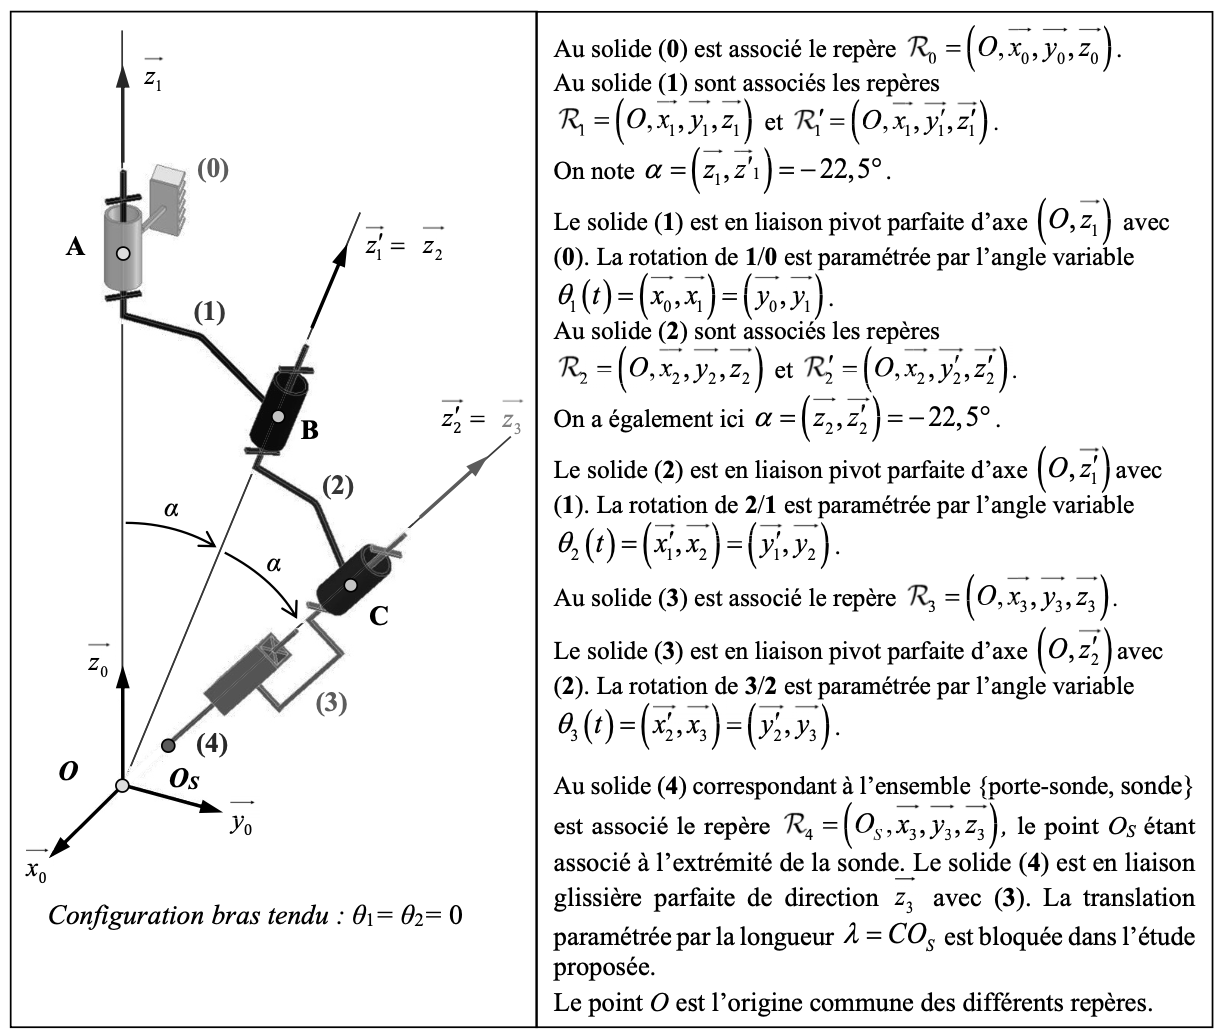
\includegraphics[width=0.9\linewidth]{img/fig05}
\end{center}
\caption{Schéma cinématique et paramétrage du robot porte-sonde configuration bras tendu}
\label{fig05}
\end{figure}

\begin{figure}[ht!]
\begin{center}
 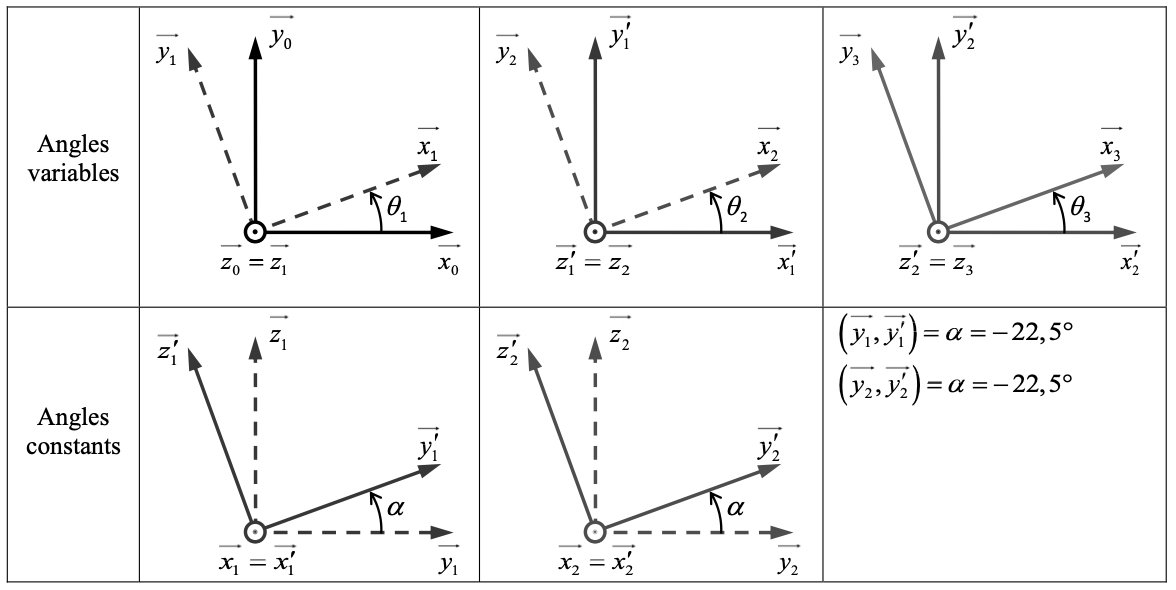
\includegraphics[width=0.9\linewidth]{img/fig06}
\end{center}
\caption{Figures de changement de base associées au robot porte-sonde}
\label{fig06}
\end{figure}


\question{Le point A est sur l'axe de rotation entre le solide 1 et le bâti 0. Déterminer $\overrightarrow{V_{O_S \in 1/0}}$ en écrivant une relation de champs de vecteurs vitesse entre les points $A$ et $O_S$ dans le mouvement de 1 par rapport au bâti (Théorème de Varignon).}

\question{Le point B est sur l'axe de rotation entre le solide 2 et le solide 1. Déterminer $\overrightarrow{V_{O_S \in 2/1}}$ en écrivant une relation de champs de vecteurs vitesse entre les points $B$ et $O_S$ dans le mouvement de 2 par rapport à 1 (Théorème de Varignon).}

\question{La translation du solide 4 par rapport à 3 est bloquée dans l'étude proposée. Déterminer alors  $\overrightarrow{V_{O_S \in 4/3}}$.}

\question{Sachant que $\overrightarrow{O_SC}=\lambda\cdot\vec{z}_3$, déterminer $\overrightarrow{V_{O_S \in 3/2}}$.}

\question{A l'aide des questions précédentes, démontrer alors que dans la configuration bras tendu, $ \overrightarrow{V_{O_s \in 4/0}}=\overrightarrow{0}$.}

\paragraph{Objectif:} Validation de l'exigence 1.1.1

\question{On rappelle que $\alpha=(\overrightarrow{z_1},\;\overrightarrow{z'_1})=(\overrightarrow{y_1},\;\overrightarrow{y'_1})=(\overrightarrow{z_2},\;\overrightarrow{z'_2})=(\overrightarrow{y_2},\;\overrightarrow{y'_2})$.
Exprimer $\overrightarrow{z'_1}$ dans la base $(\overrightarrow{x_0},\;\overrightarrow{y_0},\;\overrightarrow{z_0})$ et $\overrightarrow{z'_2}$ dans la base $(\overrightarrow{x_1},\;\overrightarrow{y_1},\;\overrightarrow{z_1})$.}

\question{En appliquant la loi de composition de mouvement sur les vecteurs vitesse de rotation, justifier, sans développer les calculs, qu'il est a priori possible d'orienter le repère $R_3$ lié à la sonde par rapport au repère $R_0$ par 3 rotations suivant les vecteurs de la base $(\overrightarrow{x_0},\;\overrightarrow{y_0},\;\overrightarrow{z_0})$.}

\question{Conclure quant à la validation de l'exigence 1.1.1}.

\subsection{Validation de l'exigence « Espace de travail » (exigence 1.1.2)}

\paragraph{Objectif:} Vérifier l'étendu de l'espace de travail (exigence 1.1.2)

\begin{figure}[ht!]
\begin{center}
 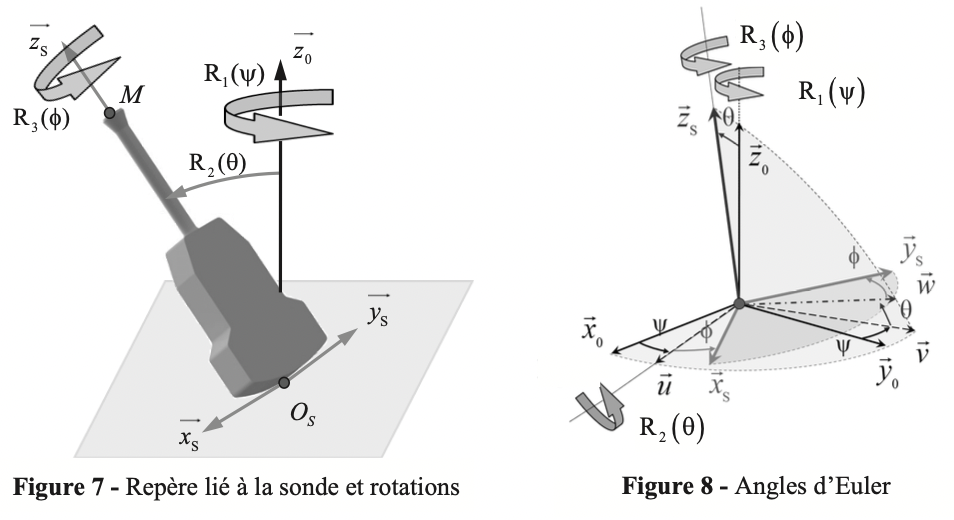
\includegraphics[width=0.9\linewidth]{img/fig07}
\end{center}
\caption{Repères liés à la sonde}
\label{fig07}
\end{figure}

L'espace de travail d'un robot est défini comme l'ensemble des positions et orientations accessibles par le repère lié à son organe terminal. En se limitant à la configuration où la sonde reste en contact avec le patient (les points $O_S$ et $O$ restent confondus), la détermination de l'espace de travail revient ici à définir l'ensemble des orientations possibles pour l'ensemble {porte-sonde, sonde}, c'est-à-dire celles du repère $R_3=(O,\;\overrightarrow{x_3},\;\overrightarrow{y_3},\;\overrightarrow{z_3})$ par rapport au repère  $R_0=(O,\;\overrightarrow{x_0},\;\overrightarrow{y_0},\;\overrightarrow{z_0})$.

\subsection{Orientation de la sonde par rapport au patient}

À la sonde (S) est associé le repère $R_S=(O,\;\overrightarrow{x_S},\;\overrightarrow{y_S},\;\overrightarrow{z_S})$ défini sur la figure \ref{fig07}. 
Ce repère est coïncidant avec le repère $R_3$. Le contact sonde/patient est assimilé à un contact ponctuel au point $O_S$. L'orientation de la sonde par rapport au patient est paramétrée par trois successives $R_1(\psi)$, $R_2(\theta)$ et $R_3(\phi)$ auxquelles sont associés les angles d'Euler $(\psi,\;\theta,\;\phi) $ (figures \ref{fig07}):
\begin{itemize}
 \item $\psi=(\overrightarrow{x_0},\overrightarrow{u})=(\overrightarrow{y_0},\overrightarrow{v})$ est associé à la rotation $R_1$ autour de $\overrightarrow{z_0}$,
 \item $\theta=(\overrightarrow{v},\overrightarrow{w})=(\overrightarrow{z_0},\overrightarrow{z_S})$ est associé à la rotation $R_2$ autour de $\overrightarrow{u}$,
 \item $\phi=(\overrightarrow{u},\overrightarrow{x_S})=(\overrightarrow{w},\overrightarrow{y_S})$ est associé à la rotation $R_3$ autour de $\overrightarrow{z_S}$.
\end{itemize}

\subsection{Élaboration d'un modèle géométrique direct partiel}

\begin{figure}[ht!]
\begin{center}
 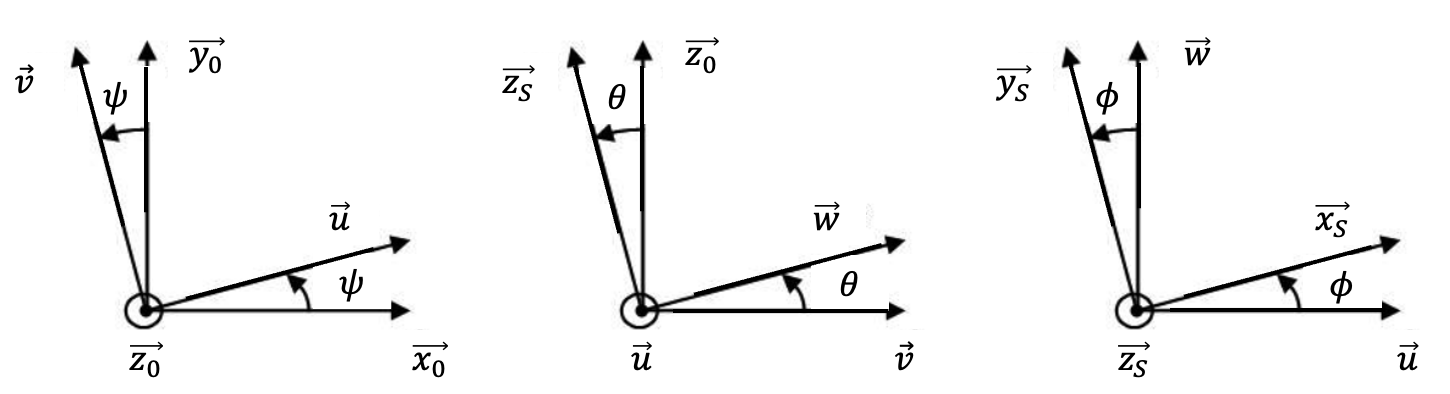
\includegraphics[width=0.9\linewidth]{img/fig08}
\end{center}
\caption{Figures de changement de repère}
\label{fig08}
\end{figure}

L'orientation de la sonde est paramétrée dans l'espace opérationnel $(X)$ par les angles $(\psi,\;\theta,\;\phi) $. Elle est liée à la configuration du robot défini quant à elle dans l'espace articulaire $(Q)$ par les angles $(\theta_1,\;\theta_2,\;\theta_3)$ paramétrant les rotations autour des axes 1, 2 et 3. La détermination de l'espace de travail nécessite d'établir la relation entre les coordonnées opérationnelle $(\psi,\;\theta,\;\phi) $, c'est-à-dire élaborer le modèle géométrique direct du robot.

\question{L'orientation de l'axe de la sonde étant définie par le vecteur $\overrightarrow{z_S}=\overrightarrow{z_3}$, déterminer les expressions des projections de ce vecteur $\overrightarrow{z_S}$ dans la base $(\overrightarrow{u},\;\overrightarrow{v},\;\overrightarrow{z_0})$ en fonction des coordonnées opérationnelles $(\theta)$,  puis dans la base $(\overrightarrow{x_0},\;\overrightarrow{y_0},\;\overrightarrow{z_0})$ en fonction des coordonnées opérationnelles $(\psi,\theta)$.}

\newpage

De la même manière, il est possible d'exprimer ce vecteur en projection dans la base $(\overrightarrow{x_0},\;\overrightarrow{y_0},\;\overrightarrow{z_0})$ en fonction des coordonnées articulaires $(\theta_1,\;\theta_2)$:

\begin{center}
$\vec{z}_3=\left(\begin{array}{c}
cos\alpha\cdot sin\alpha\cdot sin\theta_1+sin\alpha\cdot (cos\alpha\cdot sin\theta_1\cdot cos\theta_2+cos\theta_1\cdot sin\theta_2)\\
-cos\alpha\cdot sin\alpha\cdot cos\theta_1-sin\alpha\cdot (cos\alpha\cdot cos\theta_1\cdot cos\theta_2-sin\theta_1\cdot sin\theta_2)\\
cos^2\alpha-sin^2\alpha\cdot cos\theta_2
\end{array}\right)$
\end{center}

\question{Par identification des projections suivant $\overrightarrow{z_0}$, déterminer l'expression de l'angle $\theta$ en fonction de $\theta_2$ et $\alpha$. Commenter le résultat obtenu et proposer une analyse de la courbe donnée en figure \ref{fig09}.}

\question{Montrer qu'en procédant de même avec les projections suivant $\overrightarrow{x_0}$ et $\overrightarrow{y_0}$, on obtient les expressions suivantes permettant de calculer l'angle $\psi$:

\begin{eqnarray}
cos\Psi=\frac{sin\alpha\cdot (-sin\theta_1\cdot sin\theta_2+cos\alpha\cdot cos\theta_1\cdot (1+cos\theta_2))}{sin\theta}\\
sin\Psi=\frac{sin\alpha\cdot (cos\theta_1\cdot sin\theta_2+cos\alpha\cdot sin\theta_1\cdot (1+cos\theta_2))}{sin\theta}
\end{eqnarray}
}

Des relations similaires non présentées ici peuvent être obtenues pour l'angle $\phi$. L'ensemble de ces résultats permet notamment d'obtenir les courbes de la figure \ref{fig10}, qui représentent les évolutions des angles $\psi$ et $\phi$ pour $\theta_1=0^\circ$ et $\theta_2 \in [0^\circ;180^\circ[$.

\question{À partir d'une analyse des courbes obtenues, préciser en justifiant la réponse:
  \begin{enumerate}[a)]
    \item les configurations dans lesquelles se trouve le robot pour les valeurs extrêmes de l'angle $\theta$ relatives à la courbe de la figure \ref{fig09},
    \item les valeurs associées de l'angle $\beta=(\overrightarrow{x_0},\;\overrightarrow{x_S})$,
    \item la nature et les caractéristiques de la surface générée par le mouvement de l'axe de la sonde $(O,\;\overrightarrow{z_S})$.
\end{enumerate}}

\begin{figure}[ht!]
\begin{minipage}{0.45\linewidth}
\begin{center}
 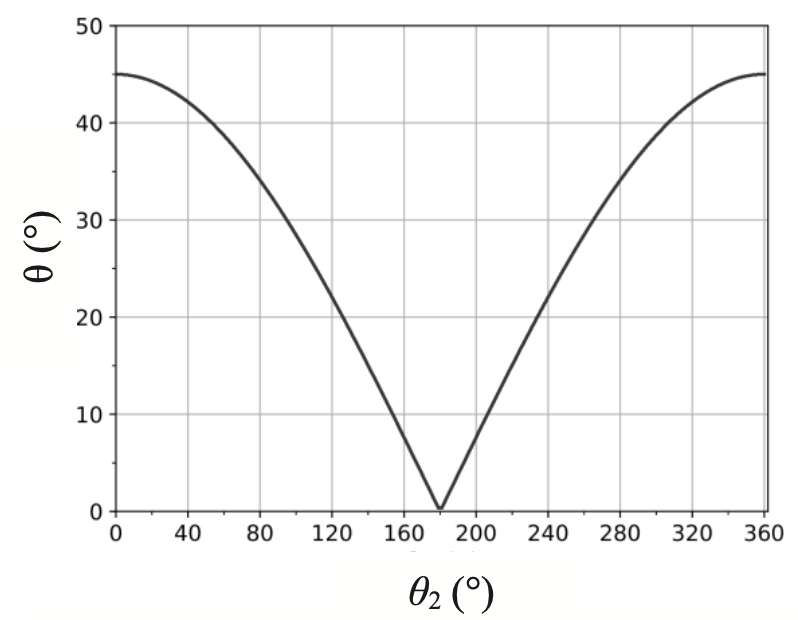
\includegraphics[width=0.9\linewidth]{img/fig09}
\end{center}
\caption{Évolution de l'angle $\theta$ en fontion du paramètre articulaire $\theta_2$}
\label{fig09}
\end{minipage}\hfill
\begin{minipage}{0.45\linewidth}
\begin{center}
 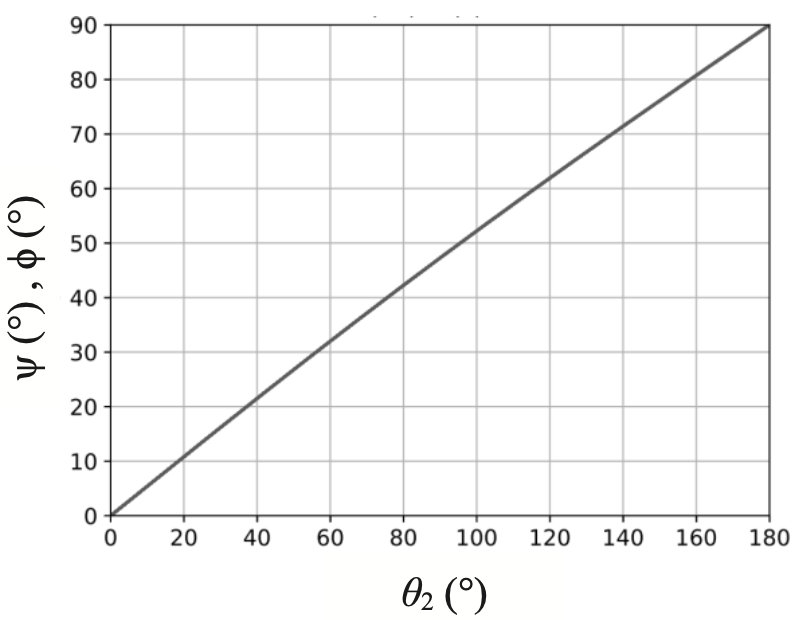
\includegraphics[width=0.9\linewidth]{img/fig10}
\end{center}
\caption{Évolution des angles $\psi$ et $\phi$ (les courbes sont ici confondues)}
\label{fig10}
\end{minipage}
\end{figure}

\subsection{Prise en compte des butées articulaires}

En pratique, l'espace de travail est limité par la présence de butées mécaniques sur les articulations, liées au contraintes de mise en \oe uvre technique. En prenant comme référence la position du robot « bras tendu », les valeurs de ces butées sont telles que pour les 2 premiers axes: $\theta_1 \in [-165^\circ,165^\circ]$, $\theta_2 \in [20^\circ,340^\circ]$. Il n'y a pas de limitation sur l'axe 3 pour lequel $\theta_3 \in [0^\circ,360^\circ]$. L'espace de travail peut être décrit à partir des positions accessibles par le point M, extrémité du vecteur unitaire $\overrightarrow{z_S}$ d'origine $O_S$, porté par l'axe de la sonde (figure \ref{fig07}). Les points de coordonnées $(z_{Sx},\;z_{Sy},\;z_{Sz})$ associés à ces positions ont été représentés sur la figure \ref{fig11} (le pas d'échantillonnage des paramètres articulaires $\theta_1$ et $\theta_2$ est de $2^\circ$) pour 2 configurations (a) et (b).

\question{A partir de l'analyse des tracés de la figure \ref{fig11}, conclure quant à la validation de l'exigence 1.1.2 liée à l'espace de travail attendu.}

~\

Soit la fonction $f$ définie de l'espace articulaire $(Q)$ vers l'espace opérationnel $(X)$, dont les applications coordonnées $(f_1,f_2)$ sont telles que $f_1(\theta_1,\theta_2)=\theta$ et $f_2(\theta_1,\theta_2)=\psi$.

\question{La fonction $f$ est-elle bijective? Justifier votre réponse en vous appuyant sur les tracés de la figure \ref{fig11} et proposer une interprétation. Quelles seront les conséquences lors de la conception de la commande du robot?}

\begin{figure}[ht!]
\begin{center}
 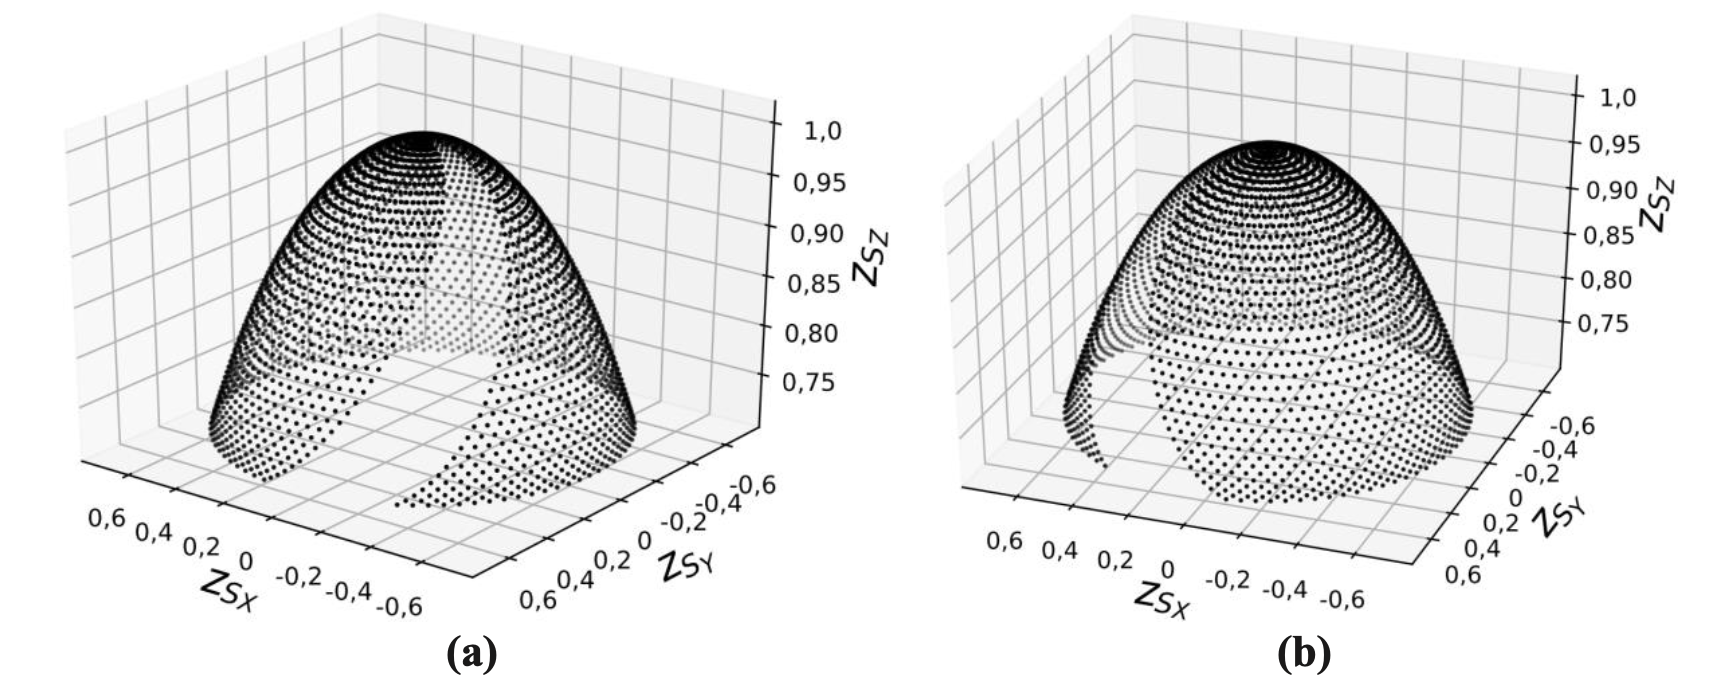
\includegraphics[width=0.9\linewidth]{img/fig11}
\end{center}
\caption{Représentation de l'espace de travail $\theta_2$ de 20 à 180° (a) et $\theta_2$ de 180 à 340° (b)}
\label{fig11}
\end{figure}

\section{Commande en position du robot porte-sonde}

\paragraph{Objectif :} Vérifier que les différentes exigences 1.2 relatives à la commande en position du robot porte-sonde peuvent être satisfaites. 

\subsection{Principe de la commande du robot porte-sonde}

La commande du robot porte-sonde repose sur la mise en \oe uvre de deux couches matérielles et logicielles qui communiquent l'une avec l'autre (figure \ref{fig12}). 

Le contrôleur haut niveau, implémenté sur le PC de contrôle du poste patient, reçoit en paramètres d'entrée, les coordonnées du positionnement désiré pour la sonde échographique, dans l'espace de travail $(\Psi,\;\theta,\;\phi)$ ainsi que les positions articulaires $(\theta_1,\;\theta_2,\;\theta_3)$ acquises par le contrôle bas-niveau. L'ensemble de ces données est traité numériquement (calcul des modèles géométriques direct et inverse du robot, prise en compte des butées articulaires, des changements d'aspect et le traitement des singularités) afin de déterminer les consignes articulaires à transmettre au contrôleur bas niveau. 

Le contrôleur bas niveau, implémenté sur la carte d'axes, reçoit les consignes articulaires et calcule les profils de vitesse $(\omega_1(t),\;\omega_2(t),\;\omega_3(t))$ transmis ensuite aux variateurs de vitesse qui pilotent les moteurs des différents axes du robot. Il assure également l'acquisition des positions articulaires qui sont communiquées au contrôleur haut niveau. 

\begin{figure}[ht!]
\begin{center}
 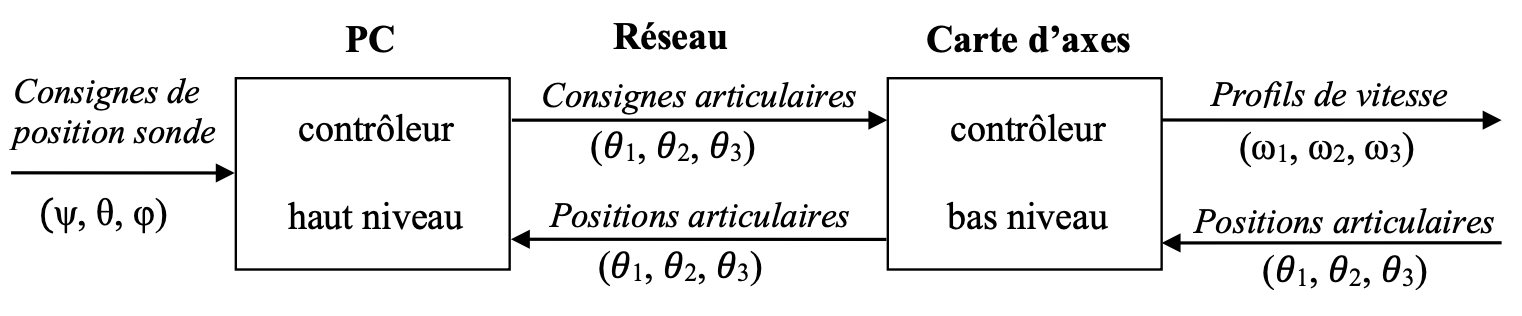
\includegraphics[width=0.9\linewidth]{img/fig12}
\end{center}
\caption{Principe de commande du robot porte-sonde}
\label{fig12}
\end{figure}

\paragraph{Commande de l'axe 1} ~\

On se limite ici à l'étude de la commande du premier axe, dont la structure est présentée en figure \ref{fig04}. Le principe associé à cette commande est décrit par la figure \ref{fig13}. La structure de commande de la position angulaire $\theta_1$ est composée de deux boucles imbriquées disposant chacune d'un réseau correcteur:
\begin{itemize}
 \item une boucle interne de vitesse, gérée par le variateur;
 \item une boucle externe de position, gérée par la carte d'axes.
\end{itemize}

\begin{figure}[ht!]
\begin{center}
 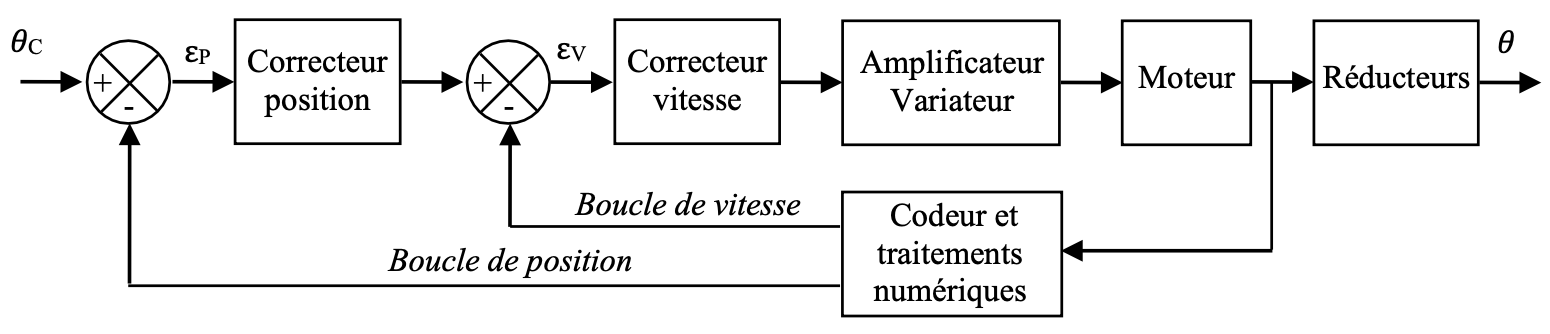
\includegraphics[width=0.9\linewidth]{img/fig13}
\end{center}
\caption{Structure de l'asservissement d'un axe}
\label{fig13}
\end{figure}

Un codeur incrémental, solidaire de l'axe moteur permet après traitement numérique d'obtenir une image de la position angulaire $\theta_1$ et de la vitesse angulaire $\omega_1$ de l'axe 1, grandeurs mises en \oe uvre au niveau des deux boucles d'asservissement. La consigne de position est élaborée par la carte d'axes, par intégration du profil de vitesse généré.

\newpage

\subsection{Modélisation de l'axe 1}

\paragraph{Objectif:} Élaborer un modèle de connaissance de l'axe 1 et réaliser la synthèse de la commande.

\paragraph{Modélisation de la motorisation} ~\ \\

On note $\Omega_m(p)$, $U(p)$, $E(p)$, $I(p)$, $C_m(p)$ et $C_{re}(p)$, les transformées de Laplace respectives de $\omega_m(t)$, $u(t)$, $e(t)$, $i(t)$, $c_m(t)$ et $c_{re}(t)$.

\begin{eqnarray}
u(t)=R\cdot i(t)+L\cdot\frac{di(t)}{dt}+e(t) \\
c_m(t)=k_c\cdot i(t) \\
e(t)=k_e\cdot\omega_m(t) \\
c_m(t)-c_{re}(t)=J_{eq}\cdot\frac{d\omega_m(t)}{dt}
\end{eqnarray}

Les différentes grandeurs intervenant dans le modèle sont définies sur la figure \ref{fig14} suivante :

\begin{figure}[ht!]
\begin{center}
 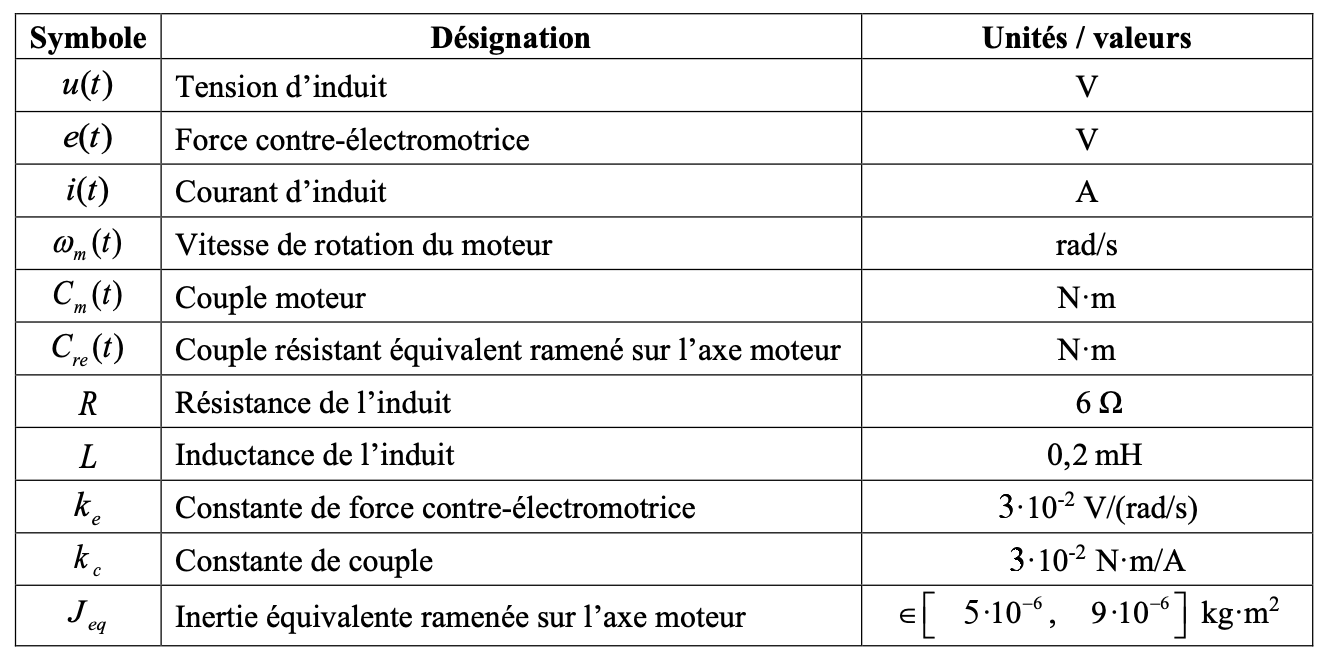
\includegraphics[width=0.9\linewidth]{img/fig14}
\end{center}
\caption{Grandeurs associées au modèle de la motorisation}
\label{fig14}
\end{figure}

\question{Déterminer les transformations de Laplace des équations (1) à (4) du moteur définies en considérant des conditions initiales nulles. Compléter les blocs correspondants sur le schéma-bloc fourni sur le document réponse par les fonctions de transfert manquantes.}

\question{Déterminer les expressions littérales des fonctions de transfert $H_1(p)=\left. \frac{\Omega_m(p)}{U(p)} \right|_{C_{re}(p)=0}$ et $H_2(p)=\left. \frac{\Omega_m(p)}{C_{re}(p)} \right|_{U(p)=0}$. Mettre sous forme canonique.}

On pose $\tau_e=\frac{L}{R}$ et $\tau_{em}=\frac{R\cdot J_{eq}}{k_e\cdot k_c}$, respectivement constantes de temps électrique et électromécanique du moteur à courant continu.

\question{Déterminer les valeurs numériques des constantes de temps $\tau_e$ et $\tau_{em}$, pour les valeurs extrêmes de $J_{eq}$. En déduire qu'une constante de temps peut être considérée comme négligeable devant l'autre.}

\question{Montrer, en précisant l'expression de $K_m$, que la fonction $H_1(p)$ peut alors de mettre sous la forme: $H_1(p)\approx\frac{K_m}{(1+\tau_e\cdot p)(1+\tau_ {em}\cdot p)}$.}

\paragraph{Modélisation de la boucle de vitesse} ~\

La figure \ref{fig15} présente la structure de la boucle de vitesse associée à la commande de l'axe 1. Pour une consigne de vitesse de rotation $\omega_c(t)$ [$m\cdot s^{-1}$], un convertisseur génère une tension de consigne de rotation à appliquer au moteur $u_{cv}(t)$ [$V$]. Un traitement numérique de la vitesse relevée sur l'axe du moteur fournit une tension mesurée $u_{mv}(t)$ [$V$], image de la vitesse de rotation du moteur $\omega_m(t)$. Un correcteur adapte le signal écart entre la tension de consigne et la tension mesurée, ce qui permet après correction et amplification, de définir la tension d'alimentation $u_m(t)$ à appliquer au moteur.

\begin{figure}[ht!]
\begin{center}
 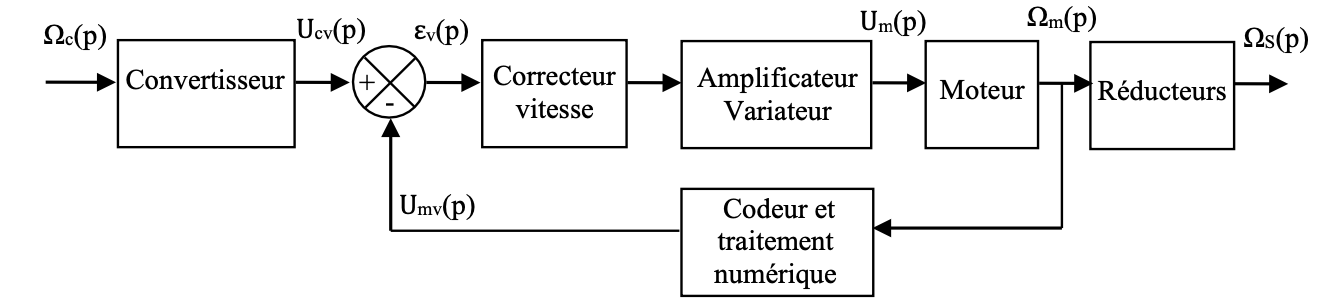
\includegraphics[width=0.9\linewidth]{img/fig15}
\end{center}
\caption{Asservissement en vitesse d'un axe}
\label{fig15}
\end{figure}

Le tableau de la figure \ref{fig16} liste les gains des différents composants intervenant dans la commande de l'axe 1.

\begin{figure}[ht!]
\begin{center}
 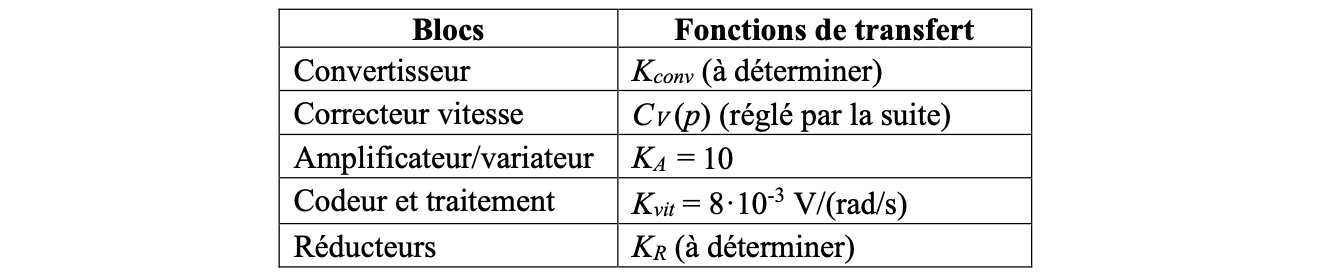
\includegraphics[width=0.9\linewidth]{img/fig16}
\end{center}
\caption{Gains des composants}
\label{fig16}
\end{figure}

On rappelle que les caractéristiques de la transmission sont définies dans le tableau 1 de la figure \ref{fig03}.

On note que $\frac{\Omega_S}{\Omega_r}=-\frac{D_1}{D_0}$ et $\frac{\Omega_r}{\Omega_m}=r$.

\question{Déterminer l'expression du gain $K_R$ (littérale). Faire l'application numérique.}

\question{Déterminer $\varepsilon_v(p)$ en fonction de $\Omega_S(p)$, $\Omega_c(p)$, $K_{conv}$, $K_{vit}$ et $K_R$. Déterminer l'expression de $K_{conv}$ pour que $\varepsilon_v(p)=0$ lorsque $\Omega_S(p)=\Omega_c(p)$. Faire l'application numérique.}

\question{Compléter le schéma-bloc sur le document réponse en y faisant figurer les fonctions de transfert sous forme littérale dans le domaine de Laplace avec des conditions initiales nulles.}

On pourrait montrer que le schéma-bloc peut se ramener au schéma à retour unitaire de la figure \ref{fig17}, avec $G_1(p)=\frac{k_c}{R}\cdot\frac{1}{1+\tau_e\cdot p}$, $G_2(p)=\frac{R}{k_c}\cdot\frac{1}{1+\tau_{em}\cdot p}$ et $K=K_{vit}\cdot K_A\cdot K_m$.

\begin{figure}[ht!]
\begin{center}
 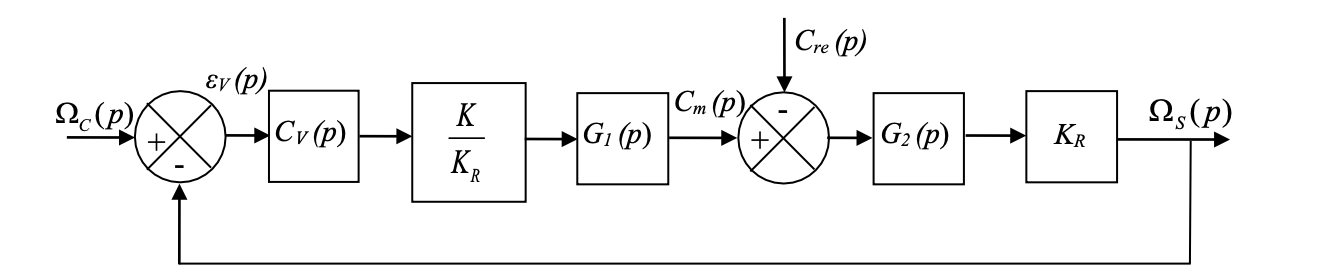
\includegraphics[width=0.9\linewidth]{img/fig17}
\end{center}
\caption{Schéma-bloc équivalent pour la boucle de vitesse}
\label{fig17}
\end{figure}

\question{A partir du schéma-bloc à retour unitaire de la figure \ref{fig17}, déterminer l'expression de la fonction de transfert en boucle ouverte $\left.H_{BO}(p)=\frac{\Omega_S(p)}{\varepsilon_V(p)}\right|_{C_{re}(p)=0}$ et de la fonction boucle fermée $\left.H_{BF}(p)=\frac{\Omega_S(p)}{\Omega_C(p)}\right|_{C_{re}(p)=0}$ en fonction de $C_V(p)$ (constante), $\tau_e$, $\tau_{em}$, $K$ et les paramètres du moteur. Indiquer la classe et l'ordre de ces 2 fonctions de transfert.}

~\

On considère une entrée $\Omega_C(p)$ en échelon, $\Omega_C(p)=\frac{\Omega_0}{p}$, avec $\Omega_0=0.1rad\cdot s^{-1}$ et $C_V(p)=1$. 

\question{Démontrer que $\varepsilon_V(p)=(1-H_{BF}(p))\cdot \Omega_C(p)$. En citant le théorème utilisé, calculer l'erreur statique $\varepsilon_s$. Discuter de la validation de l'exigence 1.2.1.1.2.}

~\

Il est nécessaire de mettre en place une action intégrale au niveau du correcteur.

\subsection{Synthèse de la commande: boucle de vitesse}

\paragraph{Objectif :} Déterminer les paramètres du correcteur de la boucle de vitesse afin de satisfaire l'exigence 1.2.1.1. 

Le système est à présent considéré en l'absence de perturbation (étude en suivi de consigne), soit $C_{re}(p)=0$. Le correcteur de la boucle de vitesse est un correcteur Proportionnel Intégral (PI), de fonction de transfert:
$C_V(p)=K_i\cdot \dfrac{1+T_i\cdot p}{T_i\cdot p}$

La constante de temps $T_i$ est choisie de manière à compenser le pôle dominant de la fonction de transfert du moteur, ce qui revient ici à prendre $T_i=\tau_{em}$. Pour l'application numérique on prendra $\tau_{em}=\tau_{em\ max}$.

\question{Déterminer en fonction des paramètres $K_i$, $K$, $\tau_{em}$ et $\tau_e$, l'expression littérale de la fonction de transfert en vitesse sous la forme canonique d'un système du second ordre:
$H_v(p)=\dfrac{\Omega_S(p)}{\Omega_C(p)}=\dfrac{K_V}{1+\dfrac{2\cdot z}{\omega_0}\cdot p+\dfrac{1}{\omega_0^2}\cdot p^2}$. Préciser la valeur de $K_V$ et les expressions littérales de z et $\omega_0$.}

~\

Le gain $K_i$ du correcteur est fixé de manière à obtenir la réponse la plus rapide sans dépassement en boucle fermée. On rappelle que pour un modèle du second ordre, la réponse la plus rapide sans dépassement est obtenue pour un facteur d'amortissement $z=1$, valeur pour laquelle on a $t_{r5\%}\omega_0 \approx 5$. On se place dans le cas où l'inertie équivalente est maximale, soit $J_{eq}=8.6 \cdot 10^{-6}\;kg \cdot m^2$.

\question{Déterminer l'expression de $K_i$ ainsi que sa valeur numérique. Déterminer la valeur du temps de réponse $t_{r5\%}$ de la boucle de vitesse pour  cette valeur de $K_i$.}

~\

On donne, sur le document réponse question \ref{q28}, le diagramme de Bode de la fonction de transfert boucle ouverte $H_{BO}(p)$ ainsi corrigée.

\question{Tracer les asymptotes sur le diagramme de Bode en Gain et sur le diagramme de Bode en phase. Déterminer alors graphiquement $H_{BO}(p)$ et ses valeurs caractéristiques.\label{q28}}

\subsection{Performances de la commande en position}

\paragraph{Objectif :} Vérifier les performances attendues pour la boucle de position (exigence 1.2.1.2.). 

Les performances de la boucle de vitesse étant validées, on complète le modèle numérique avec la boucle de position (figure 13). Les paramètres du correcteur Proportionnel Intégral Dérivé (PID) de la boucle de position sont déterminés à l'aide de l'outil de simulation numérique. La réponse temporelle en position de l'axe 1, pour une consigne en échelon de $10^\circ$, est représentée sur la figure du document réponse, question \ref{q29}.

\question{En faisant apparaître les constructions, déterminer graphiquement le temps de réponse à $5\%$ du système. Conclure quant au respect de l'exigence 1.2.1.2.\label{q29}}

\section{Lecture de plan}

\question{Sur le dessin du document réponse, colorier les différentes classes d'équivalence du système.}

\vspace{2cm}

\begin{center}
\Huge{Fin de l'épreuve}
\end{center}

\newpage

\section{Annexe}

\begin{figure}[ht!]
\begin{center}
 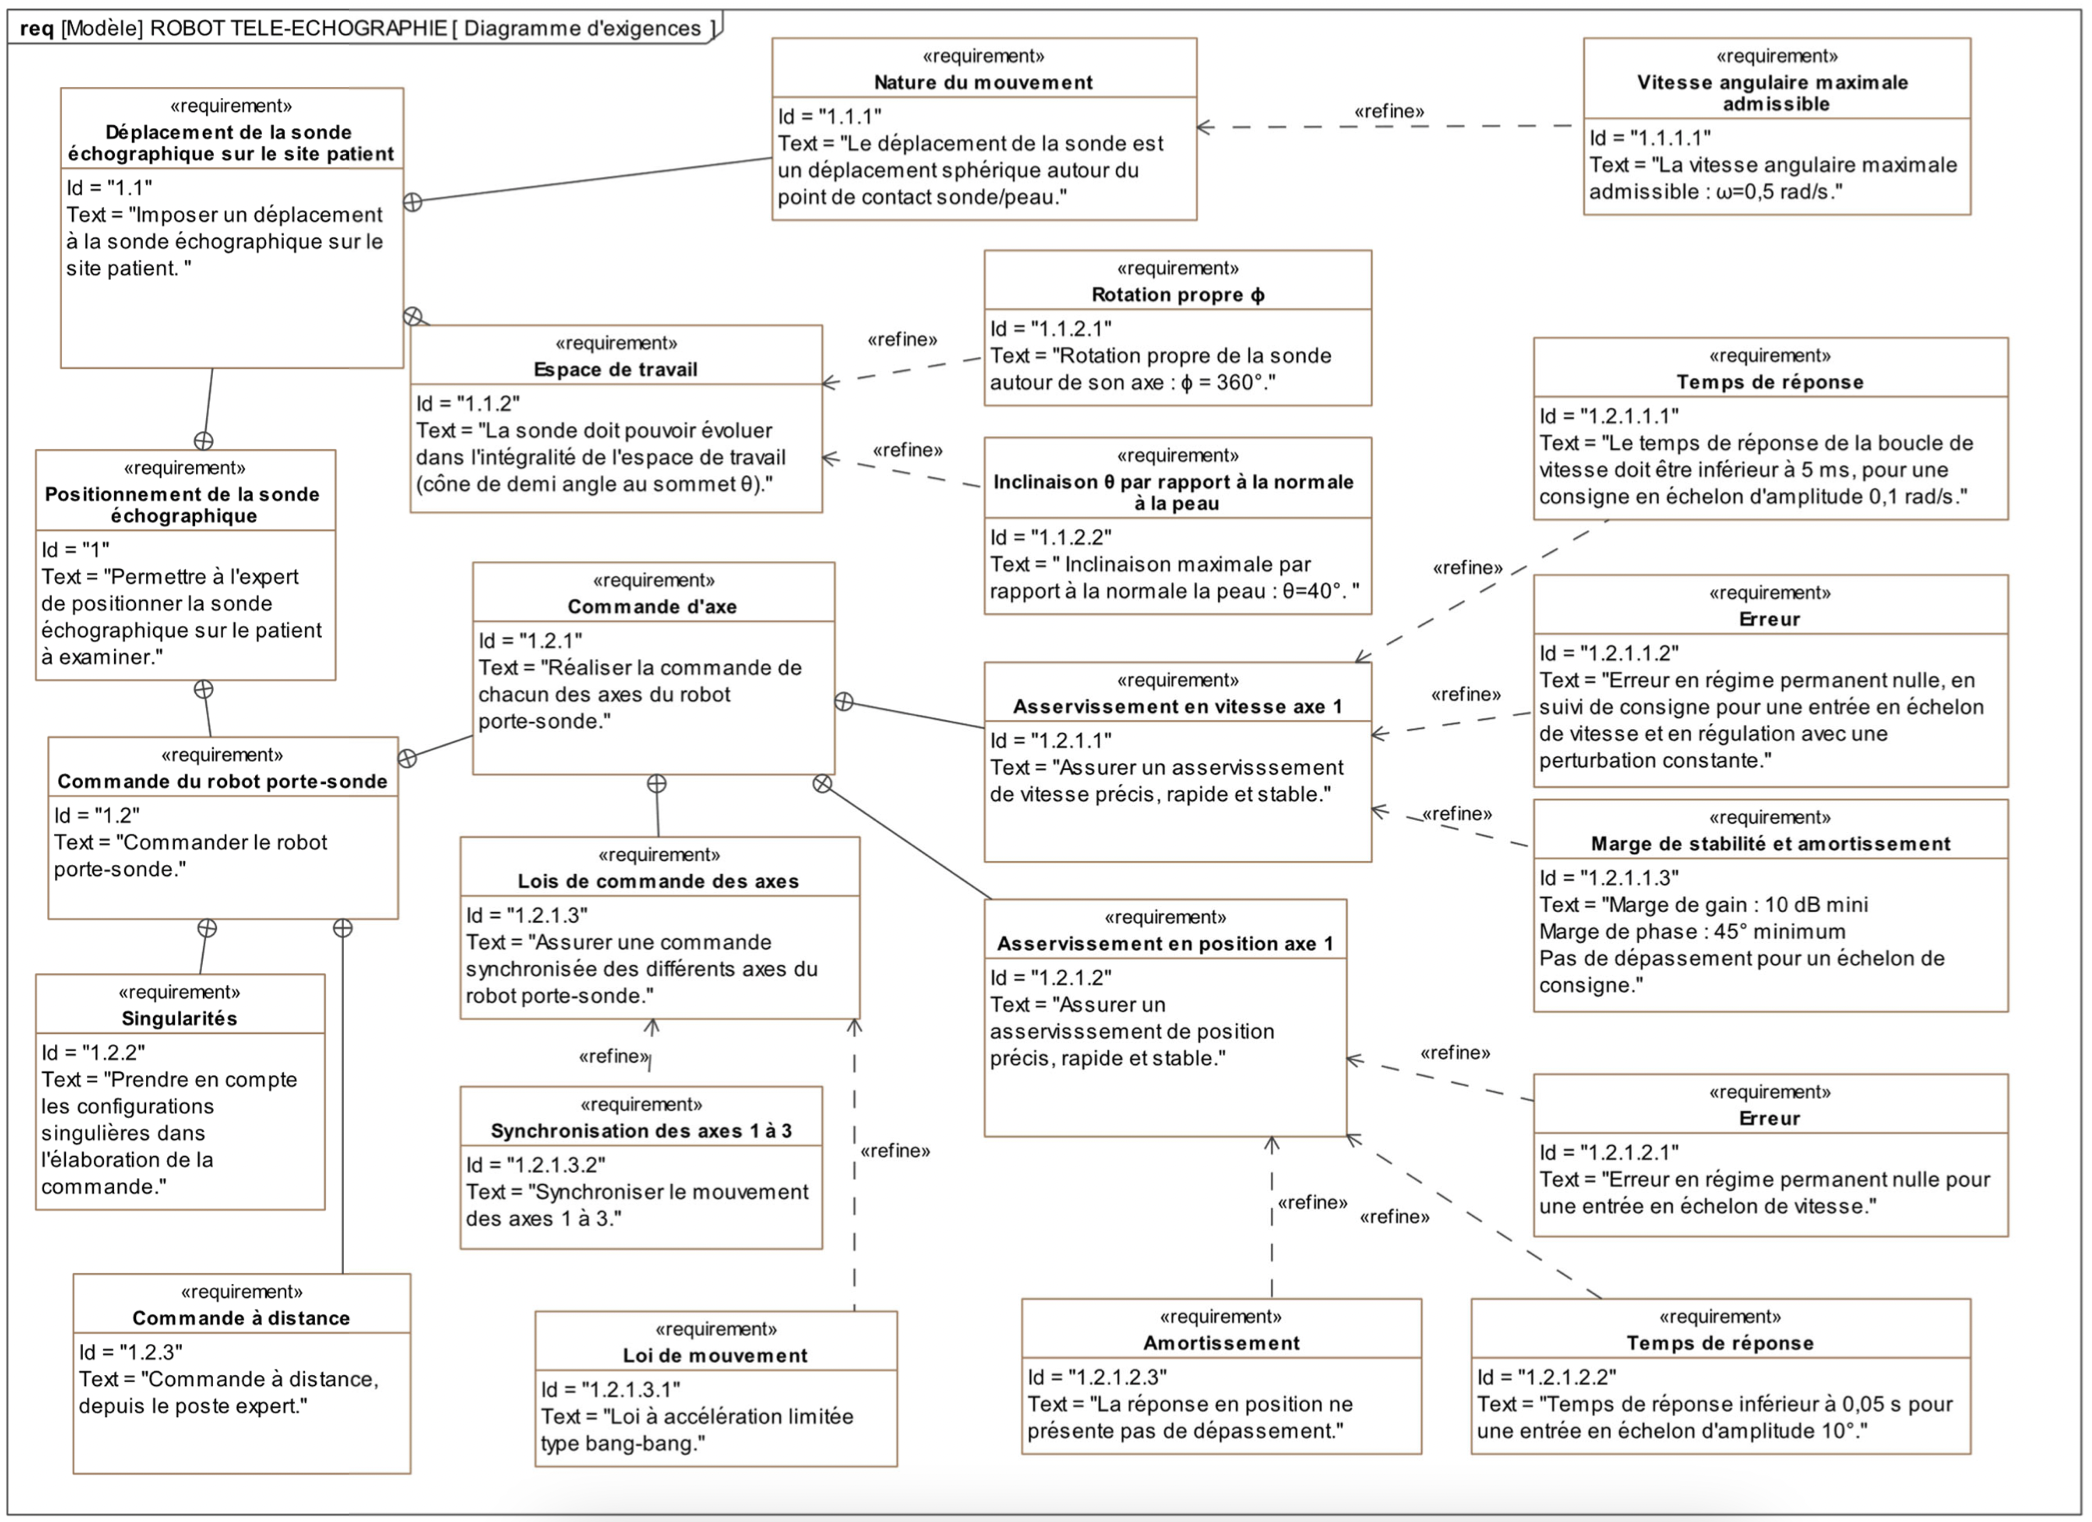
\includegraphics[width=0.9\linewidth]{img/exigences}
\end{center}
\caption{Diagramme d'exigences}
\label{exigences}
\end{figure}


\cleardoublepage

\ifdef{\public}{\pagestyle{documentreponse}}{\pagestyle{correction}}

\reponse{2}{}{$\overrightarrow{V_{O_S\in4/0}}=\overrightarrow{V_{O_S\in4/3}}+\overrightarrow{V_{O_S\in3/2}}+\overrightarrow{V_{O_S\in2/1}}+\overrightarrow{V_{O_S\in1/0}}$}

\reponse{3}{}{$\overrightarrow{\Omega_{1/0}}=\dot{\theta_1}\cdot \vec{z_0}$,$\overrightarrow{\Omega_{2/1}}=\dot{\theta_2}\cdot \vec{z'_1}$. Dans la configuration bras tendu, $\theta_1$ et $\theta_2$ sont constants, donc $\overrightarrow{\Omega_{1/0}}=\vec{0}$ et $\overrightarrow{\Omega_{2/1}}=\vec{0}$}

\reponse{3}{}{$\overrightarrow{V_{O_S\in1/0}}=\overrightarrow{V_{A\in1/0}}+\overrightarrow{O_SA}\wedge\overrightarrow{\Omega_{1/0}}=\overrightarrow{V_{A\in1/0}}$ car $\overrightarrow{O_SA}$ et $\overrightarrow{\Omega_{1/0}}$ sont colinéaires, donc $\overrightarrow{V_{O_S\in1/0}}=\vec{0}$}

\reponse{3}{}{$\overrightarrow{V_{O_S\in2/1}}=\overrightarrow{V_{B\in2/1}}+\overrightarrow{O_SB}\wedge\overrightarrow{\Omega_{2/1}}=\overrightarrow{V_{B\in2/1}}$ car $\overrightarrow{O_SB}$ et $\overrightarrow{\Omega_{2/1}}$ sont colinéaires, donc $\overrightarrow{V_{O_S\in1/0}}=\vec{0}$}

\reponse{2}{}{Si la translation est bloquée alors $\overrightarrow{V_{O_S\in4/3}}=\vec{0}$}

\ifdef{\public}{\newpage}

\reponse{2}{}{$\overrightarrow{V_{O_S\in3/2}}=\left[\frac{d\overrightarrow{CO_S}}{dt}\right]_{R_2}=-\left[\frac{d\lambda\cdot\vec{z_3}}{dt}\right]_{R_2}=-\lambda\cdot\overrightarrow{\Omega_{3/2}}\wedge\vec{z_3}=\vec{0}$ car $\overrightarrow{\Omega_{3/2}}$ et $\vec{z_3}$ sont colinéaires.}

\reponse{2}{}{On obtient donc $\overrightarrow{V_{O_S\in4/0}}=\vec{0}$.}

\reponse{4}{}{$\vec{z'_1}=-sin\alpha\cdot\vec{y_1}+cos\alpha\cdot\vec{z_1}$

$\vec{z'_1}=-sin\alpha\cdot(-sin\theta_1\cdot\vec{x_0}+cos\theta_1\cdot\vec{y_0})+cos\alpha\cdot\vec{z_0}$

$\vec{z'_1}=sin\alpha\cdot sin\theta_1\cdot\vec{x_0}-sin\alpha\cdot cos\theta_1\cdot\vec{y_0}+cos\alpha\cdot\vec{z_0}$

De même, 
$\vec{z'_2}=sin\alpha\cdot sin\theta_2\cdot\vec{x'_1}-sin\alpha\cdot cos\theta_2\cdot\vec{y'_1}+cos\alpha\cdot\vec{z'_1}=sin\alpha\cdot sin\theta_2\cdot\vec{x_1}-sin\alpha\cdot cos\alpha\cdot(1+cos\theta2)\cdot\vec{y_1}+(cos^2\alpha-cos\theta_2\cdot sin^2\alpha)\cdot\vec{z_1}$
}

\reponse{4}{}{$\overrightarrow{\Omega_{3/0}}=\overrightarrow{\Omega_{3/2'}}+\overrightarrow{\Omega_{2'/2}}+\overrightarrow{\Omega_{2/1'}}+\overrightarrow{\Omega_{1'/1}}+\overrightarrow{\Omega_{1/0}}=\dot{\theta_3}.\vec{z_3}+\dot{\theta_2}.\vec{z_2}+\dot{\theta_1}.\vec{z_1}$.

$\vec{z_1}=\vec{z_0}$, $\vec{z_3}$ et $\vec{z_2}$ s'écrivent en fonction de $\vec{x_0}$, $\vec{y_0}$ et $\vec{z_0}$.
}

\reponse{2}{}{Comme il y a trois rotations indépendantes, le mouvement est bien sphérique.}

\ifdef{\public}{\newpage}

\reponse{4}{}{$\vec{z_S}=-sin\theta\cdot\vec{v}+cos\theta\cdot\vec{z_0}$

$\vec{z_S}=-sin\theta\cdot(-sin\psi\cdot\vec{x_0}+cos\psi\cdot\vec{y_0})+cos\theta\cdot\vec{z_0}$

$\vec{z_S}=sin\theta\cdot sin\psi\cdot\vec{x_0}-sin\theta\cdot cos\psi\cdot\vec{y_0}+cos\theta\cdot\vec{z_0}$}

\reponse{6}{}{$cos\theta=cos^2\alpha-sin^2\alpha\cdot cos\theta_2$

$\theta=arccos\left(cos^2\alpha-sin^2\alpha\cdot cos\theta_2\right)$

On voit que:
\begin{itemize}
 \item $\theta_2=180^\circ \Rightarrow \theta=arccos(1)=0^\circ$
 \item $\theta(\theta_2)=\theta(-\theta_2)$, donc il y a une symétrie par rapport à $\theta_2=180^\circ$,
 \item si $\theta_2=0$, alors $\theta=arccos\left(cos^2\alpha-sin^2\alpha\right)=arccos\left(cos(2\cdot\alpha)\right)=2\cdot22.5=45^\circ$
\end{itemize} 
}


\reponse{7}{}{
$sin\theta\cdot sin\psi=cos\alpha\cdot sin\alpha\cdot sin\theta_1+sin\alpha\cdot (cos\alpha\cdot sin\theta_1\cdot cos\theta_2+cos\theta_1\cdot sin\theta_2)$

$sin\psi=\dfrac{sin\alpha\cdot (cos\alpha\cdot sin\theta_1\cdot (1+cos\theta_2)+cos\theta_1\cdot sin\theta_2)}{sin\theta}$

$cos\psi=\dfrac{cos\alpha\cdot sin\alpha\cdot cos\theta_1+sin\alpha\cdot (cos\alpha\cdot cos\theta_1\cdot cos\theta_2-sin\theta_1\cdot sin\theta_2)}{sin\theta}$

$cos\psi=\dfrac{sin\alpha\cdot (cos\alpha\cdot cos\theta_1\cdot (1+cos\theta_2)-sin\theta_1\cdot sin\theta_2)}{sin\theta}$
}

\ifdef{\public}{\newpage}

\reponse{4}{}{
\begin{enumerate}[a)]
 \item $\theta=0$: $\theta_2=180$ (bras replié), $\psi=\phi=90$
 $\theta=45$, $\theta_2=0$ (bras tendu), $\psi=\phi=0$,
 \item $\theta=0$: $\vec{x_0}=-\vec{v}$, $\vec{v}=\vec{w}$, $\vec{x_S}=\vec{w}$, donc $\beta=180^\circ$,
 $\theta=45$: $\vec{x_0}=\vec{u}$, $\vec{x_S}=\vec{u}$, donc $\beta=0^\circ$,
 \item La surface balayée par l'axe de la sonde appartient à un cône de révolution de sommet O et d'axe $(O,\vec{z_2})$
\end{enumerate}
}

\reponse{3}{}{
L'espace de travail complet est obtenu en sommant les deux espaces de la figure \ref{fig11}. On constate qu'il y a recouvrement sauf pour une zone proche de (0.1,0.4,0.7). On peut cependant supposer que cette zone n'est pas nécessaire pour satisfaire le cahier des charges.}

\reponse{3}{}{
En sachant qu'il y a recouvrement pour la majorité des coordonnées, la fonction n'est pas bijective, il y a plusieurs antécédents pour une même image. Il faudra donc le prendre en compte dans la commande pour que les variations se fassent de manière continue.}

\reponse{4}{\begin{center}
 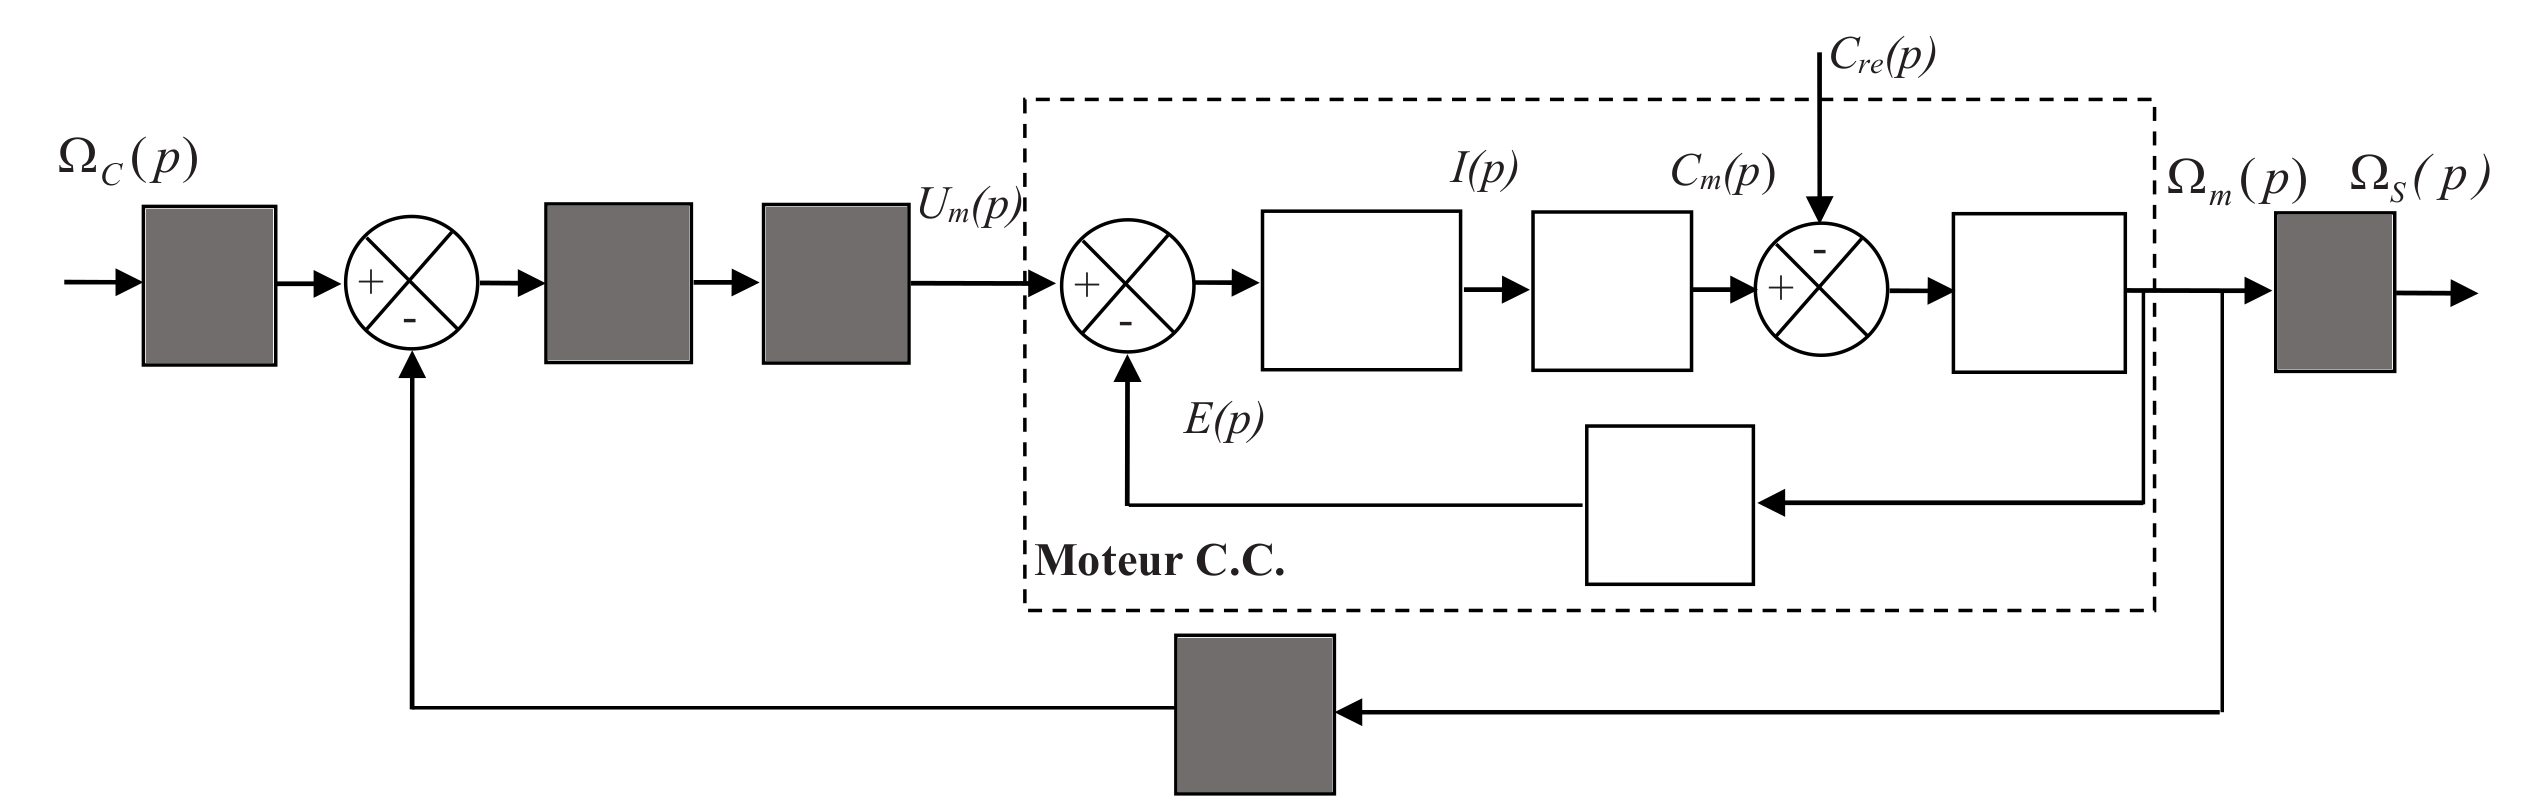
\includegraphics[width=0.9\linewidth]{img/DR01}
\end{center}}{

\begin{eqnarray}
U(p)=R\cdot I(p)+L\cdot p\cdot I(p)+E(p) \\
C_m(p)=k_c\cdot I(p) \\
E(p)=k_e\cdot\Omega_m(p) \\
C_m(p)-C_{re}(p)=J_{eq}\cdot p\cdot\Omega_m(p)
\end{eqnarray}

\begin{center}
 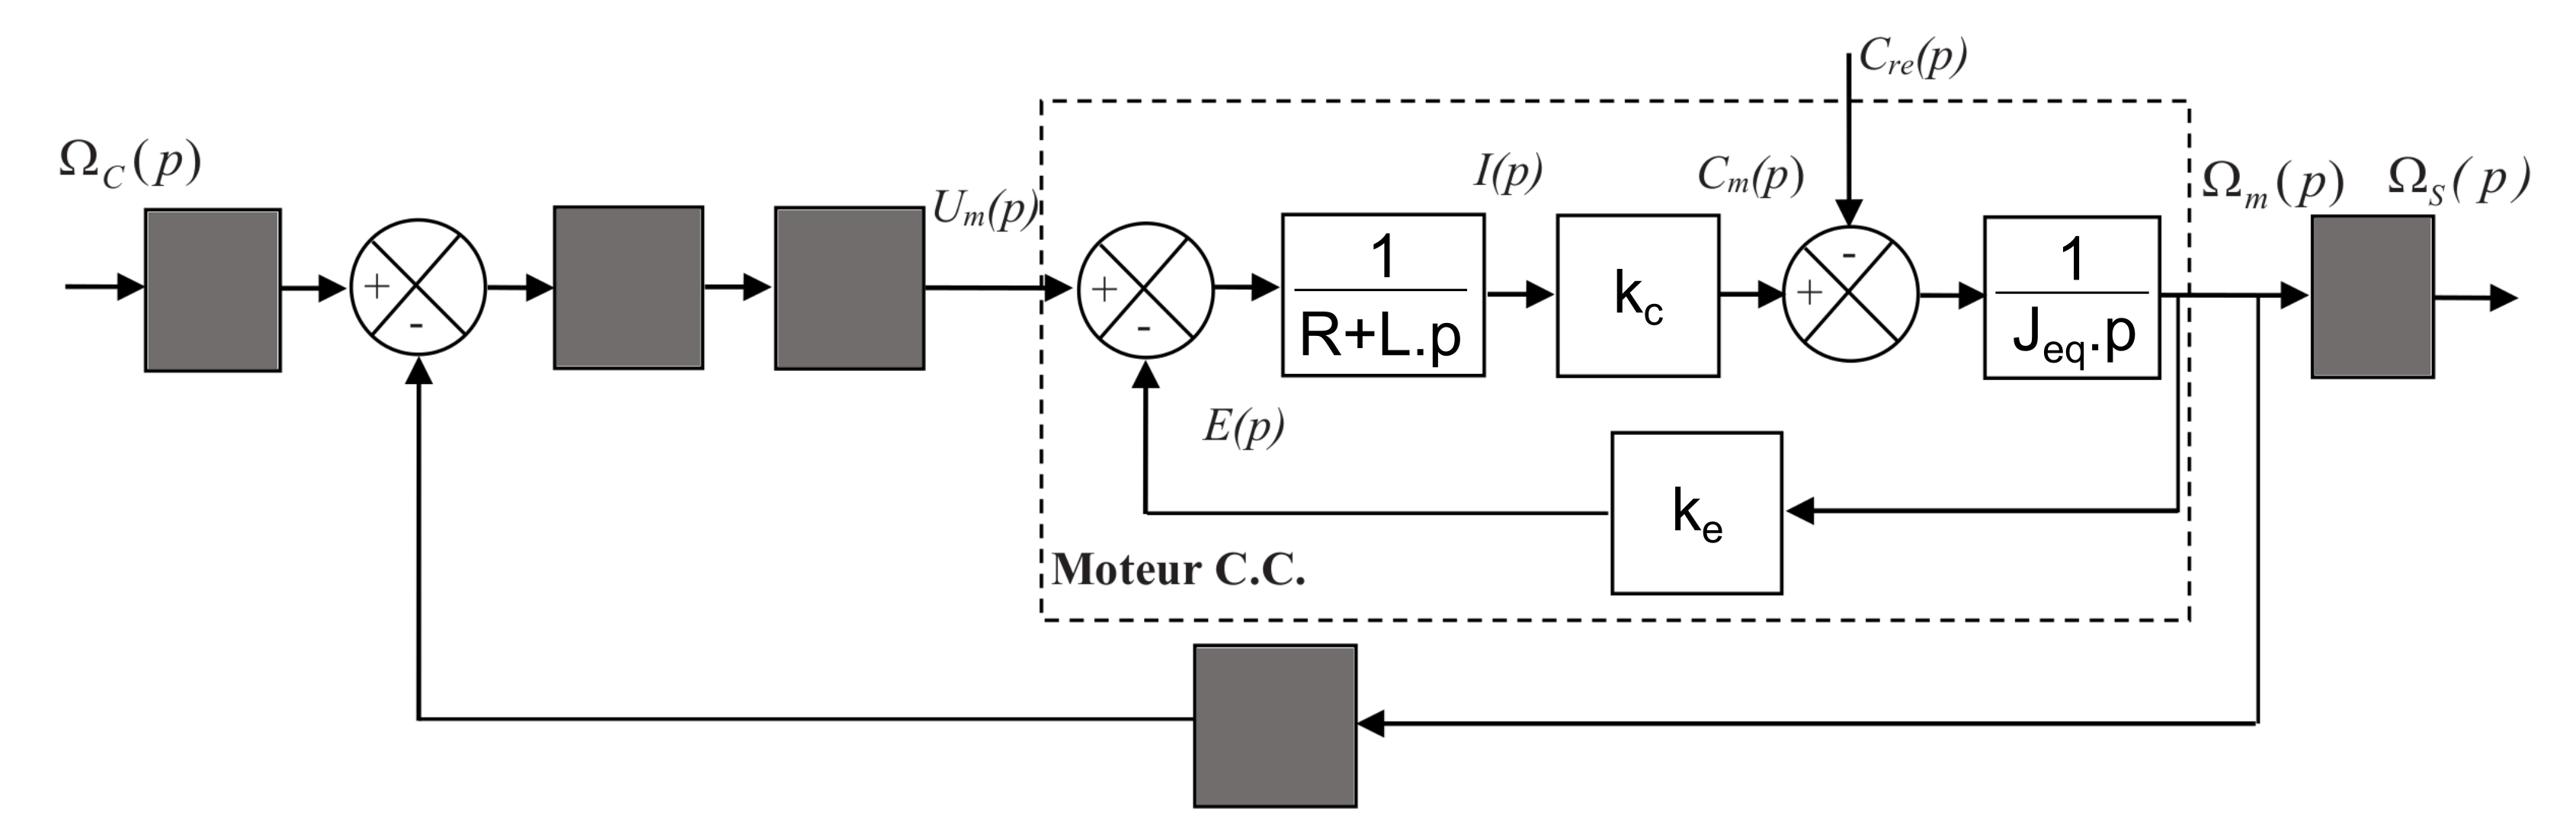
\includegraphics[width=0.9\linewidth]{img/DR01_cor}
\end{center}
}

\reponse{8}{}{
$H_1(p)=\left. \dfrac{\Omega_m(p)}{U(p)} \right|_{C_{re}(p)=0}=\dfrac{\dfrac{1}{R+L\cdot p}\cdot k_c\cdot \dfrac{1}{J_{eq}\cdot p}}{1+\dfrac{1}{R+L\cdot p}\cdot k_c\cdot \dfrac{1}{J_{eq\cdot p}}\cdot k_e}=\dfrac{k_c}{J_{eq}\cdot p\cdot(R+L\cdot p)+k_c\cdot k_e}$

$H_1(p)=\dfrac{\dfrac{1}{k_e}}{1+\dfrac{J_{eq}\cdot R}{k_c\cdot k_e}\cdot p+\dfrac{J_{eq}\cdot L}{k_c\cdot k_e}\cdot p^2}$

$H_2(p)=\left. \dfrac{\Omega_m(p)}{C_{re}(p)} \right|_{U(p)=0}$

$I(p)=\dfrac{-E(p)}{R+L\cdot p}$

$C_m(p)=k_c\cdot \dfrac{-k_e\cdot\Omega_m(p)}{R+L\cdot p}$

$\left[k_c\cdot \dfrac{-k_e}{R+L\cdot p}-J_{eq}\cdot p\right]\cdot\Omega_m(p)=C_{re}(p)$

$\dfrac{\Omega_m(p)}{C_{re}(p)}=-\dfrac{R+L\cdot p}{k_c\cdot k_e+J_{eq}\cdot p\cdot (R+L\cdot p)}$

$H_2(p)=-\dfrac{R}{k_c\cdot k_e}\cdot\dfrac{1+\dfrac{L}{R}\cdot p}{1+\dfrac{J_{eq}\cdot R}{k_c\cdot k_e}\cdot p+\dfrac{J_{eq}\cdot L}{k_c\cdot k_e}\cdot p^2}$

}

\reponse{6}{}{
$\tau_e=\dfrac{L}{R}=\dfrac{2\cdot 10^{-4}}{6}\approx 3\cdot 10^{-5}\approx 0.03 ms$

$\dfrac{6\cdot 5\cdot 10^{-6}}{3^2 \cdot 10^{-4}}\leq\tau_{em}\leq\dfrac{6\cdot 9\cdot 10^{-6}}{3^2 \cdot 10^{-4}}$

$\dfrac{6\cdot 5\cdot 10^{-6}}{9 \cdot 10^{-4}}\leq\tau_{em}\leq\dfrac{6\cdot 9\cdot 10^{-6}}{9 \cdot 10^{-4}}$

$\dfrac{5}{3}\cdot 10^{-4}\leq\tau_{em}\leq 6\cdot 10^{-2}$

$0.017\leq\tau_{em}\leq 0.06$

Donc, $\tau_e$ est négligeable devant $\tau_{em}$.
}

\ifdef{\public}{\newpage}

\reponse{6}{}{
$H_1(p)=\dfrac{\dfrac{1}{k_e}}{1+\dfrac{J_{eq}\cdot R}{k_c\cdot k_e}\cdot p+\dfrac{L}{R}\cdot\dfrac{J_{eq}\cdot R}{k_c\cdot k_e}\cdot p^2}=\dfrac{\dfrac{1}{k_e}}{1+\tau_{em}\cdot p+\tau_e\cdot\tau_{em}\cdot p^2}$

Or $\dfrac{\dfrac{1}{k_e}}{(1+\tau_{em}\cdot p)\cdot(1+\tau_e\cdot p)}=\dfrac{\dfrac{1}{k_e}}{1+(\tau_{em}+\tau_e)\cdot p+\tau_e\cdot\tau_{em}\cdot p^2}$ et comme $\tau_{e}<<\tau_{em}$, on peut écrire

$H_1(p)\approx\dfrac{\dfrac{1}{k_e}}{(1+\tau_{em}\cdot p)\cdot(1+\tau_e\cdot p)}$

Donc $K_m=\frac{1}{k_e}$
}

\reponse{2}{}{
$K_R=\frac{\Omega_S(p)}{\Omega_m(p)}=-\frac{D_1}{D_0}\cdot r=-\frac{12}{48}\cdot \frac{1}{30}=-\frac{1}{120}\approx -0.008$}


\reponse{3}{}{$\varepsilon_v(p)=U_{cv}(p)-U_{mv}(p)=\Omega_C(p)\cdot K_{conv}-\Omega_m(p)\cdot K_{vit}$

$\varepsilon_v(p)=\Omega_C(p)\cdot K_{conv}-\Omega_S(p)\cdot \frac{K_{vit}}{K_R}$

$0=\Omega_S(p)\cdot K_{conv}-\Omega_S(p)\cdot \frac{K_{vit}}{K_R}$

$0=K_{conv}-\frac{K_{vit}}{K_R}$

Donc $K_{conv}=\frac{K_{vit}}{K_R}$

$K_{conv}=-\frac{8\cdot 10^{-3}}{8\cdot 10^{-3}}=-1$
}

\reponse{0}{\begin{center}
 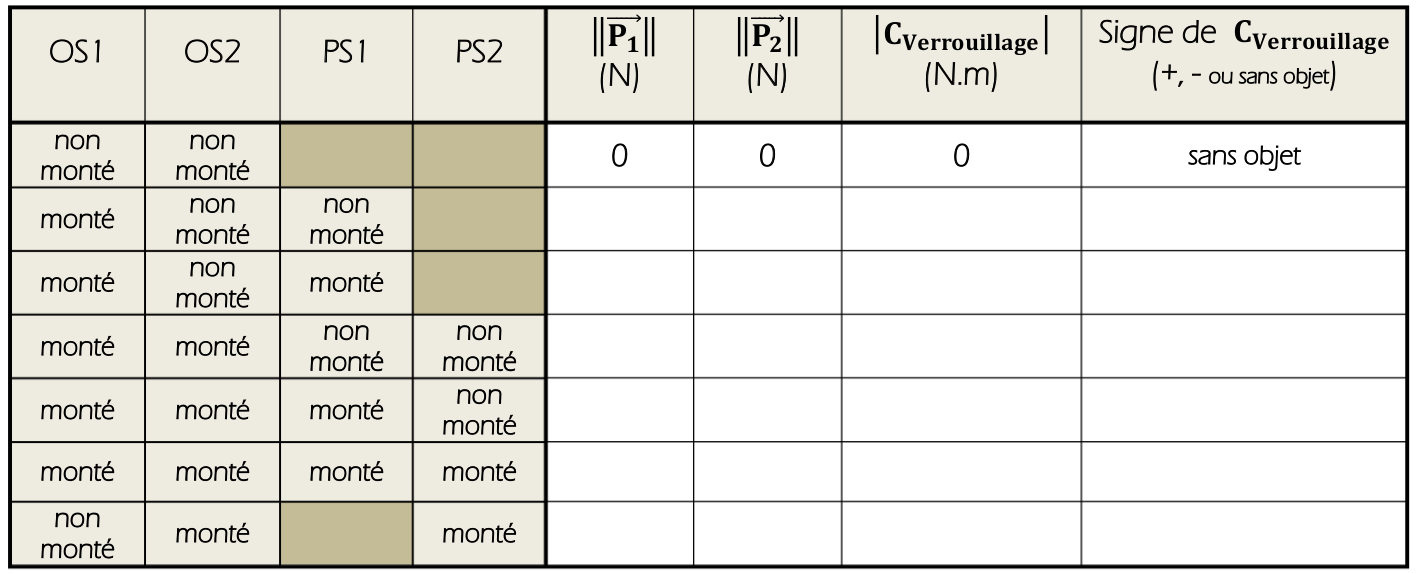
\includegraphics[width=0.9\linewidth]{img/DR02}
\end{center}}{
\begin{center}
 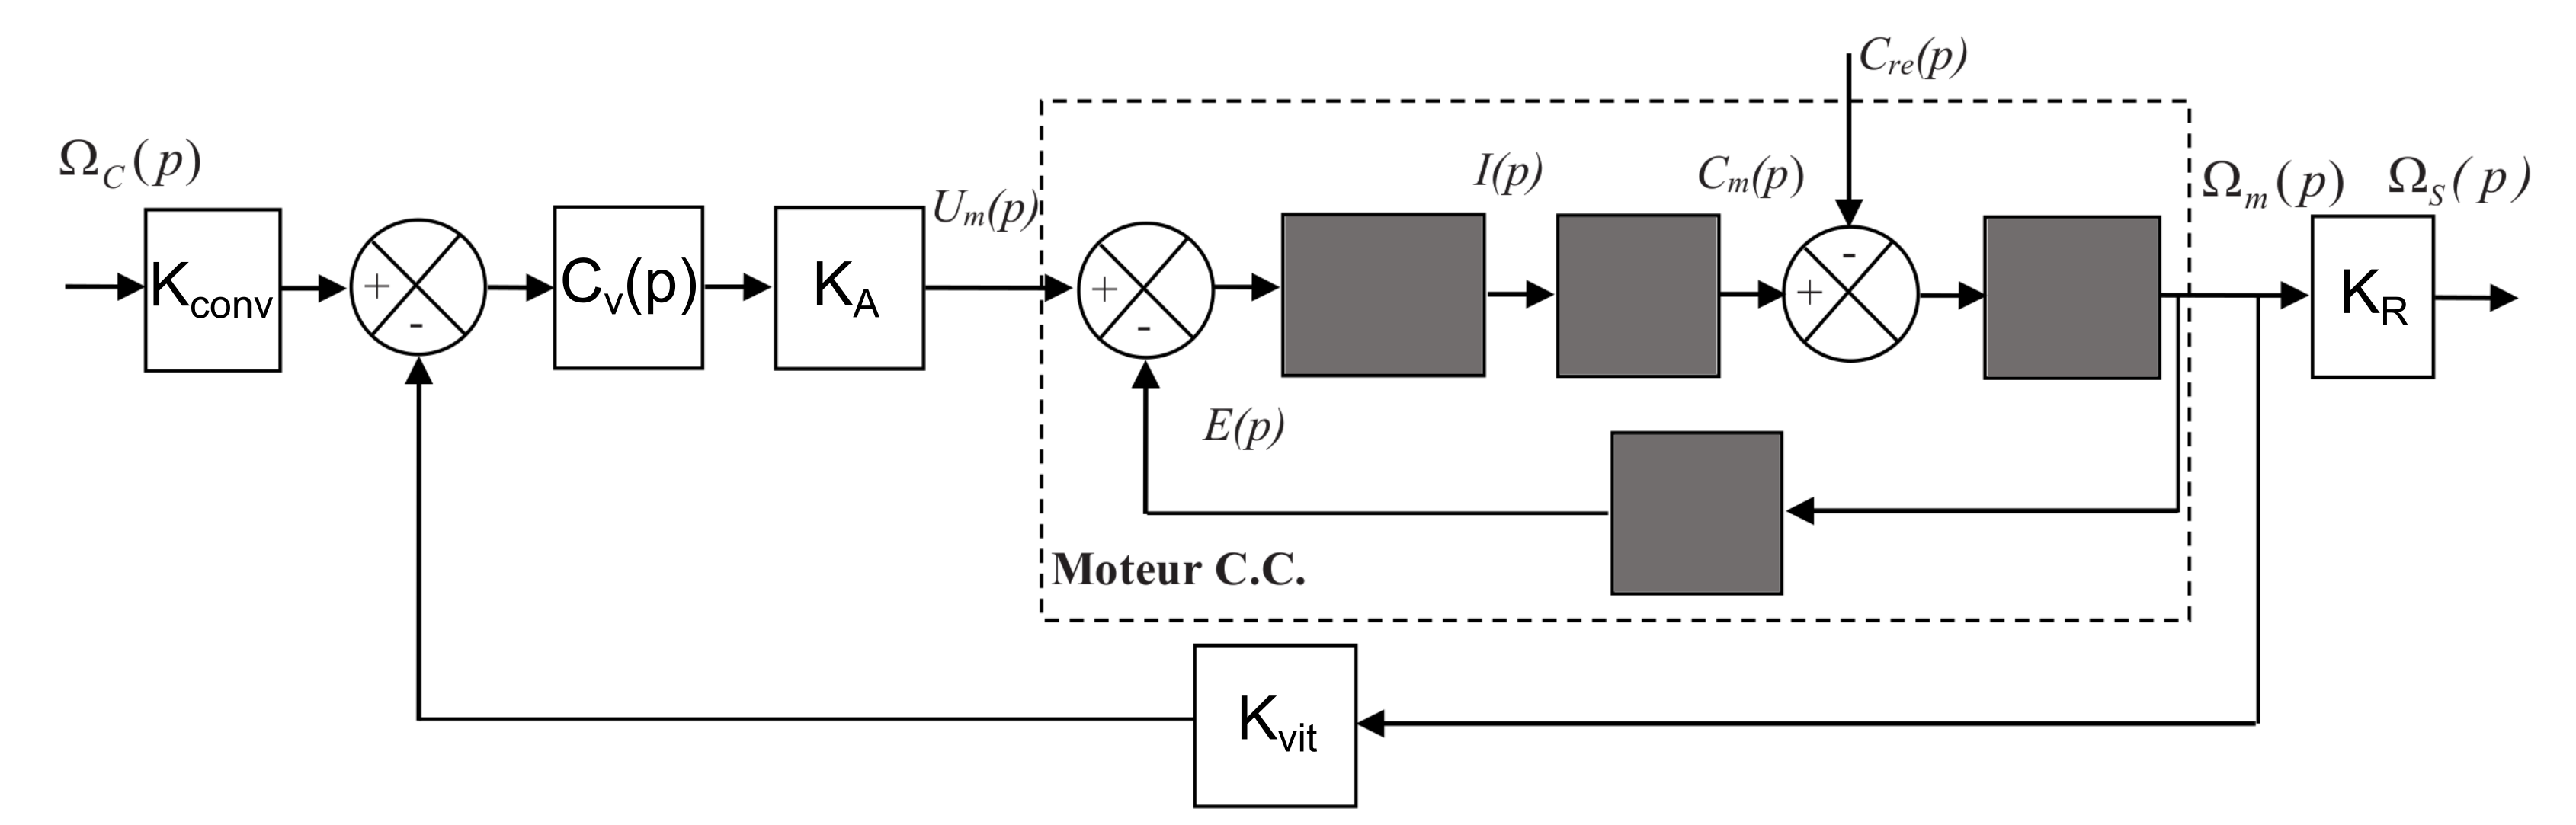
\includegraphics[width=0.9\linewidth]{img/DR02_cor}
\end{center}}

\ifdef{\public}{\vspace{-1cm}}

\reponse{6}{}{$H_{BO}(p)=C_V(p)\cdot\dfrac{K}{K_R}\cdot G_1(p)\cdot G_2(p)\cdot K_R=C_V(p)\cdot\dfrac{K}{K_R}\cdot \dfrac{k_c}{R}\cdot\dfrac{1}{1+\tau_e\cdot p}\cdot \dfrac{R}{k_c}\cdot\dfrac{1}{1+\tau_{em}\cdot p}\cdot K_R$

$H_{BO}(p)=\dfrac{C_V(p)\cdot K}{(1+\tau_e\cdot p)\cdot(1+\tau_{em}\cdot p)}$

Fonction d'ordre 2 et de classe 0.

$H_{BF}(p)=\dfrac{C_V(p)\cdot\dfrac{K}{K_R}\cdot G_1(p)\cdot G_2(p)\cdot K_R}{1+{C_V(p)\cdot\dfrac{K}{K_R}\cdot G_1(p)\cdot G_2(p)\cdot K_R}}$

$H_{BF}(p)=\dfrac{C_V(p)\cdot\dfrac{K}{K_R}\cdot \dfrac{k_c}{R}\cdot\dfrac{1}{1+\tau_e\cdot p}\cdot \dfrac{R}{k_c}\cdot\dfrac{1}{1+\tau_{em}\cdot p}\cdot K_R}{1+{C_V(p)\cdot\dfrac{K}{K_R}\cdot \dfrac{k_c}{R}\cdot\dfrac{1}{1+\tau_e\cdot p}\cdot \dfrac{R}{k_c}\cdot\dfrac{1}{1+\tau_{em}\cdot p}\cdot K_R}}$

$H_{BF}(p)=\dfrac{C_V(p)\cdot K\cdot \dfrac{1}{1+\tau_e\cdot p}\cdot\dfrac{1}{1+\tau_{em}\cdot p}}{1+{C_V(p)\cdot K\cdot \dfrac{1}{1+\tau_e\cdot p}\cdot\dfrac{1}{1+\tau_{em}\cdot p}}}$

$H_{BF}(p)=\dfrac{C_V(p)\cdot K}{(1+\tau_e\cdot p)\cdot(1+\tau_{em}\cdot p)+{C_V(p)\cdot K}}$

Fonction d'ordre 2 et de classe 0.
}

\reponse{6}{}{
$\varepsilon_v(p)=\Omega_c(p)-\Omega_S(p)=\Omega_c(p)-\dfrac{\Omega_S(p)}{\Omega_c(p)}\cdot\Omega_c(p)=(1-H_{BF}(p))\cdot\Omega_c(p)$

D'après le théorème de la valeur finale, \[\varepsilon_S=\lim_{p\to 0} p\cdot \varepsilon_v(p)=\lim_{p\to 0} p\cdot (1-H_{BF}(p))\cdot\Omega_c(p) \]

\[\lim_{p\to 0} H_{BF}(p)=\dfrac{K}{1+K}\]

\[\varepsilon_S=\left(1-\dfrac{K}{1+K}\right)\cdot\Omega_0=\dfrac{\Omega_0}{1+K}\]

$K=K_{vit}\cdot K_A\cdot K_m=\dfrac{8\cdot 10^{-3}\cdot 10}{3\cdot 10^{-2}}=\dfrac{8}{3}\approx 2.66$

\[\varepsilon_S\approx\dfrac{0.1}{1+2.66}\approx 0.03rad.s^{-1}\]
}

\reponse{6}{}{
$H_V(p)=\dfrac{K_i\cdot \dfrac{1+T_i\cdot p}{T_i\cdot p}\cdot K}{(1+\tau_e\cdot p)\cdot(1+\tau_{em}\cdot p)+{K_i\cdot \dfrac{1+T_i\cdot p}{T_i\cdot p}\cdot K}}$

$H_V(p)=\dfrac{K_i\cdot \dfrac{1+\tau_{em}\cdot p}{\tau_{em}\cdot p}\cdot K}{(1+\tau_e\cdot p)\cdot(1+\tau_{em}\cdot p)+{K_i\cdot \dfrac{1+\tau_{em}\cdot p}{\tau_{em}\cdot p}\cdot K}}$

$H_V(p)=\dfrac{K_i\cdot \dfrac{1}{\tau_{em}\cdot p}\cdot K}{(1+\tau_e\cdot p)+{K_i\cdot \dfrac{1}{\tau_{em}\cdot p}\cdot K}}$

$H_V(p)=\dfrac{K_i\cdot K}{(1+\tau_e\cdot p)\cdot \tau_{em}\cdot p+{K_i\cdot K}}$

$H_V(p)=\dfrac{1}{1+\frac{\tau_{em}}{K_i\cdot K}\cdot p+\frac{\tau_{em}\cdot \tau_e}{K_i\cdot K}\cdot p^2}$

Donc,

\begin{eqnarray}
K_V=1 \\
\omega_0=\sqrt{\frac{K_i\cdot K}{\tau_{em}\cdot \tau_e}} \\
\xi=\frac{1}{2}\cdot\sqrt{\frac{\tau_{em}}{K_i\cdot K\cdot \tau_e}}
\end{eqnarray}
}

\ifdef{\public}{\newpage}

\reponse{6}{}{
La réponse la plus rapide sans dépassement existe pour $\xi=\dfrac{1}{2}\cdot\sqrt{\dfrac{\tau_{em}}{K_i\cdot K\cdot \tau_e}}=1$

$\dfrac{\tau_{em}}{K_i\cdot K\cdot \tau_e}=2^2$

$K_i=\dfrac{\tau_{em}}{4\cdot K\cdot \tau_e}$

$K_i=\dfrac{0.06}{4\cdot 2.66\cdot 3\cdot 10^{-5}}\approx\dfrac{3\cdot 10^3}{16}\approx 200$

$\omega_0=\sqrt{\frac{200\cdot 2.66}{0.06\cdot 3\cdot 10^{-5}}}=\sqrt{\frac{8\cdot 10^9}{27}}\approx 1,7\cdot 10^4 rad.s^{-1}$

Donc, $tr_{5\%}=\dfrac{5}{1,7\cdot 10^4}\approx 0.3ms$
}

\reponse{4}{\begin{center}
 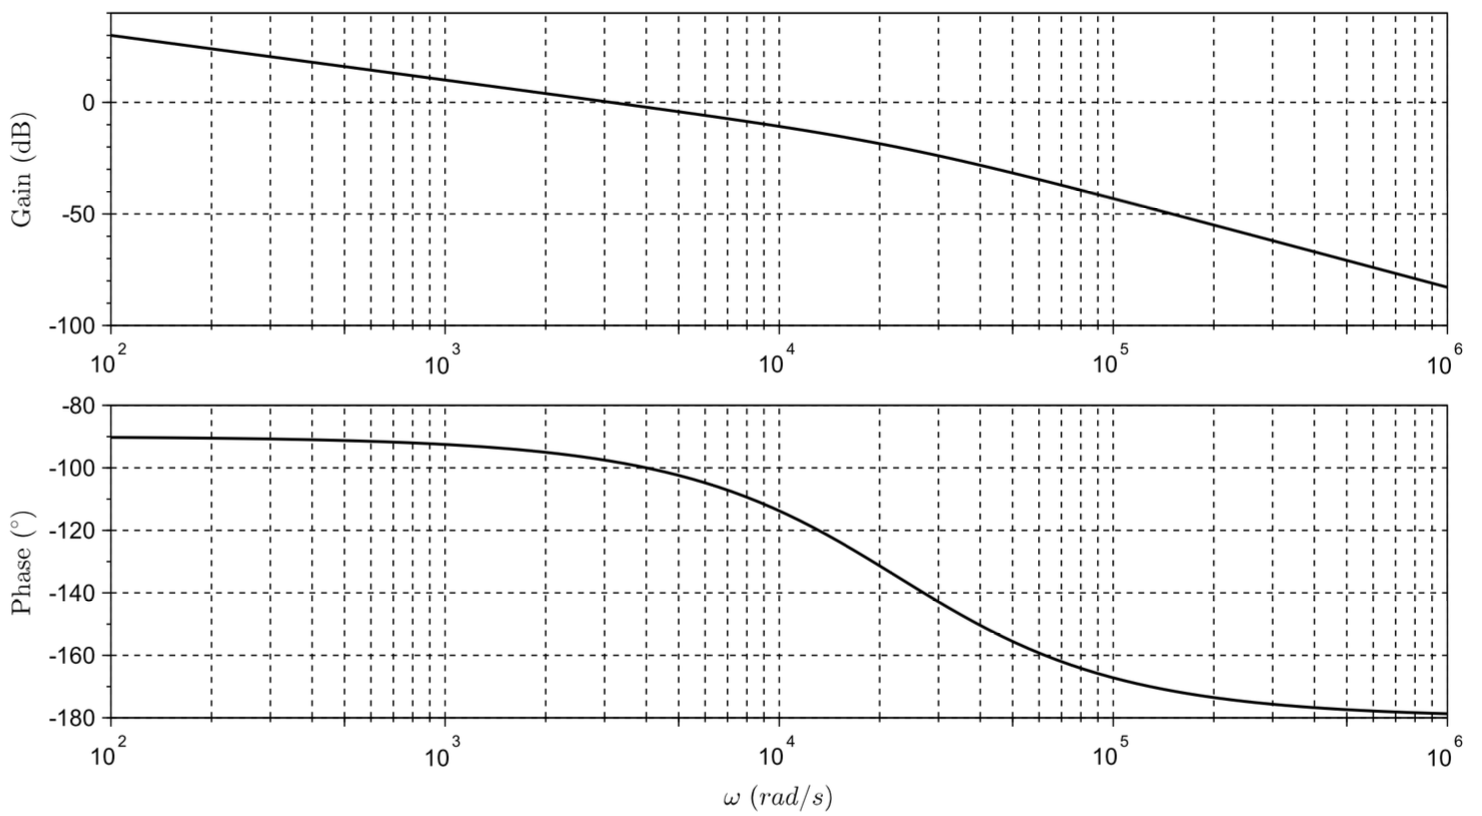
\includegraphics[width=0.9\linewidth]{img/DR03}
\end{center}}{
\begin{center}
 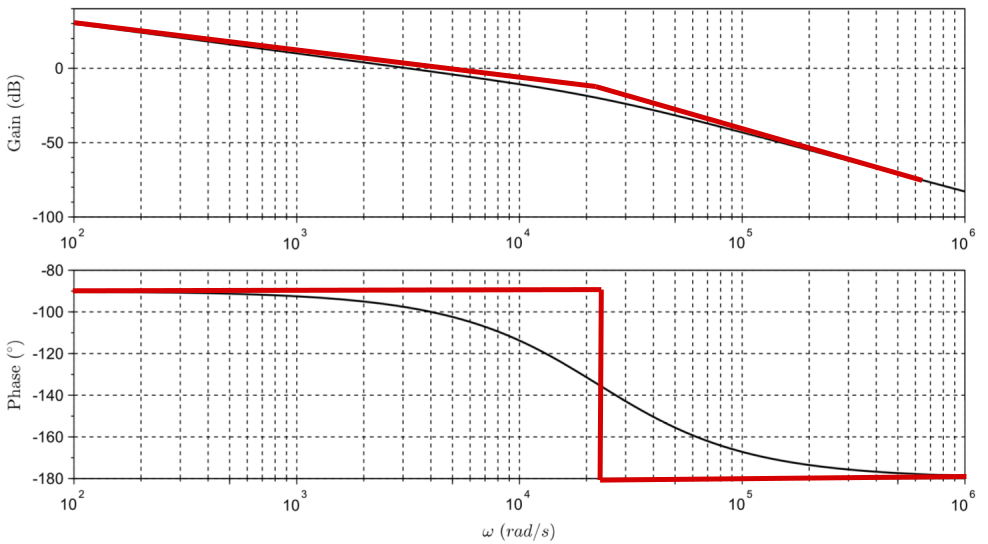
\includegraphics[width=0.9\linewidth]{img/DR03_cor}
\end{center}

C'est une fonction de transfert d'ordre 2 et de classe 1, la pulsation de cassure est $\omega_c=21000rad.s^{-1}$, donc $\tau_c=\frac{1}{21000}\approx 5\cdot 10^{-5}s$

Pour $\omega=10^3rad.s^{-1}$, $20\cdot log(K)-20\cdot log(\omega)=10$, donc $20\cdot log(K)=10+20*3=70$

$log(K)=3.5$, donc $K=10^{3.5}\approx 1000*3=3000$
}

\ifdef{\public}{\vfill\newpage}

\reponse{2}{\begin{center}
 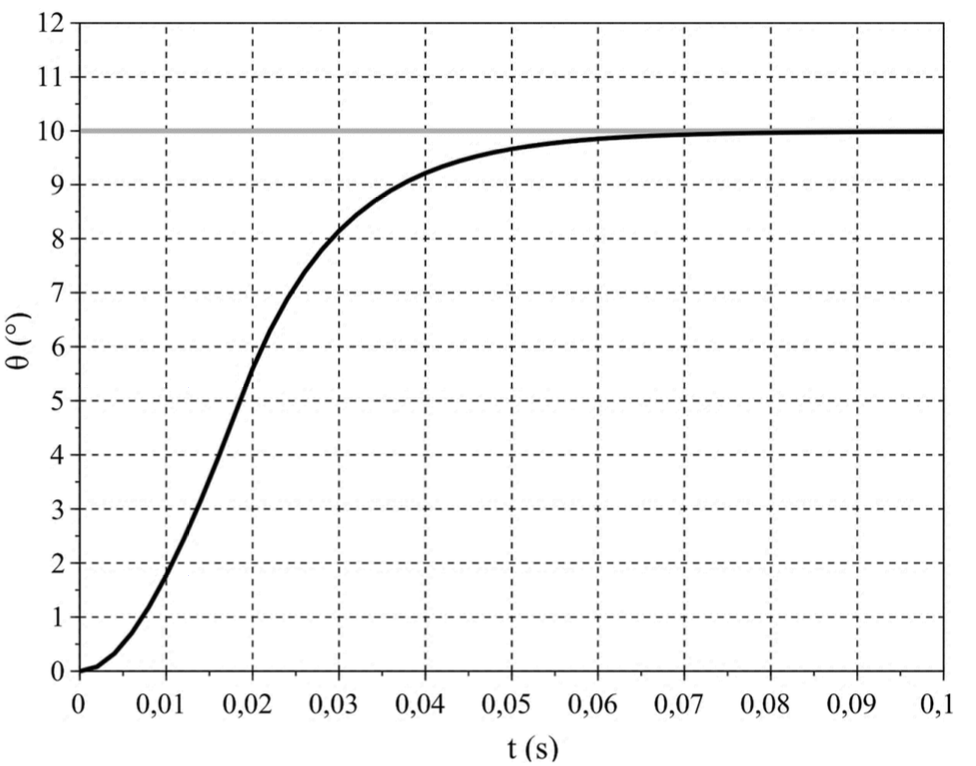
\includegraphics[width=0.8\linewidth]{img/DR04}
\end{center}}{
\begin{center}
 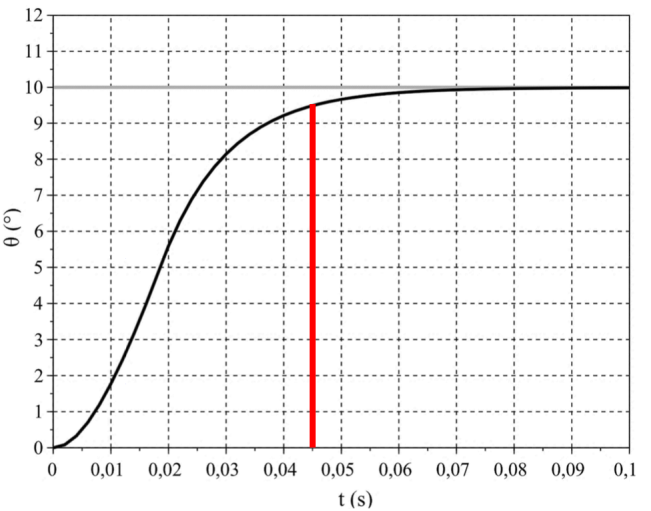
\includegraphics[width=0.8\linewidth]{img/DR04_cor}
\end{center}
Le temps de réponse est de $0.045s$.
}

\ifdef{\public}{\vfill\newpage}

\reponse{0}{\begin{center}
 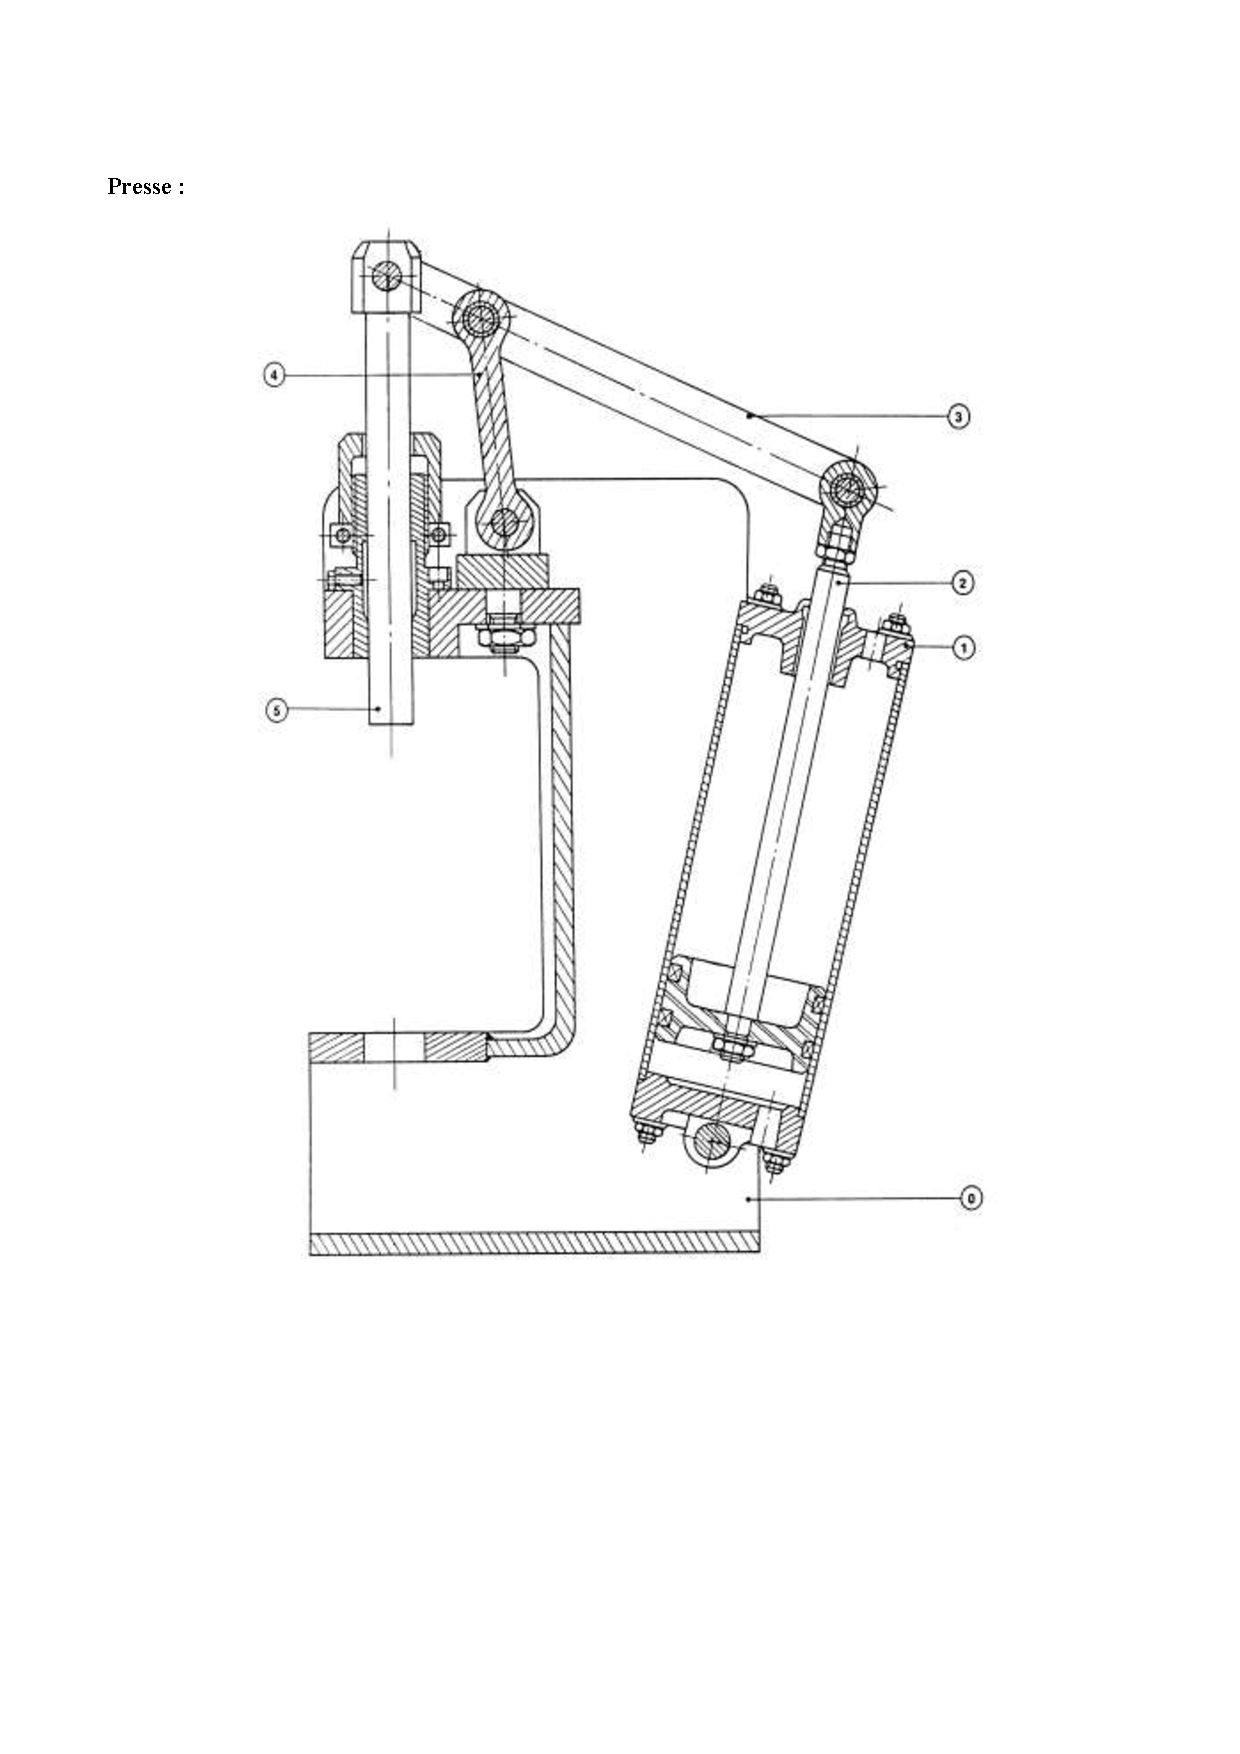
\includegraphics[width=0.95\linewidth]{img/DR05}
\end{center}}{
\begin{center}
 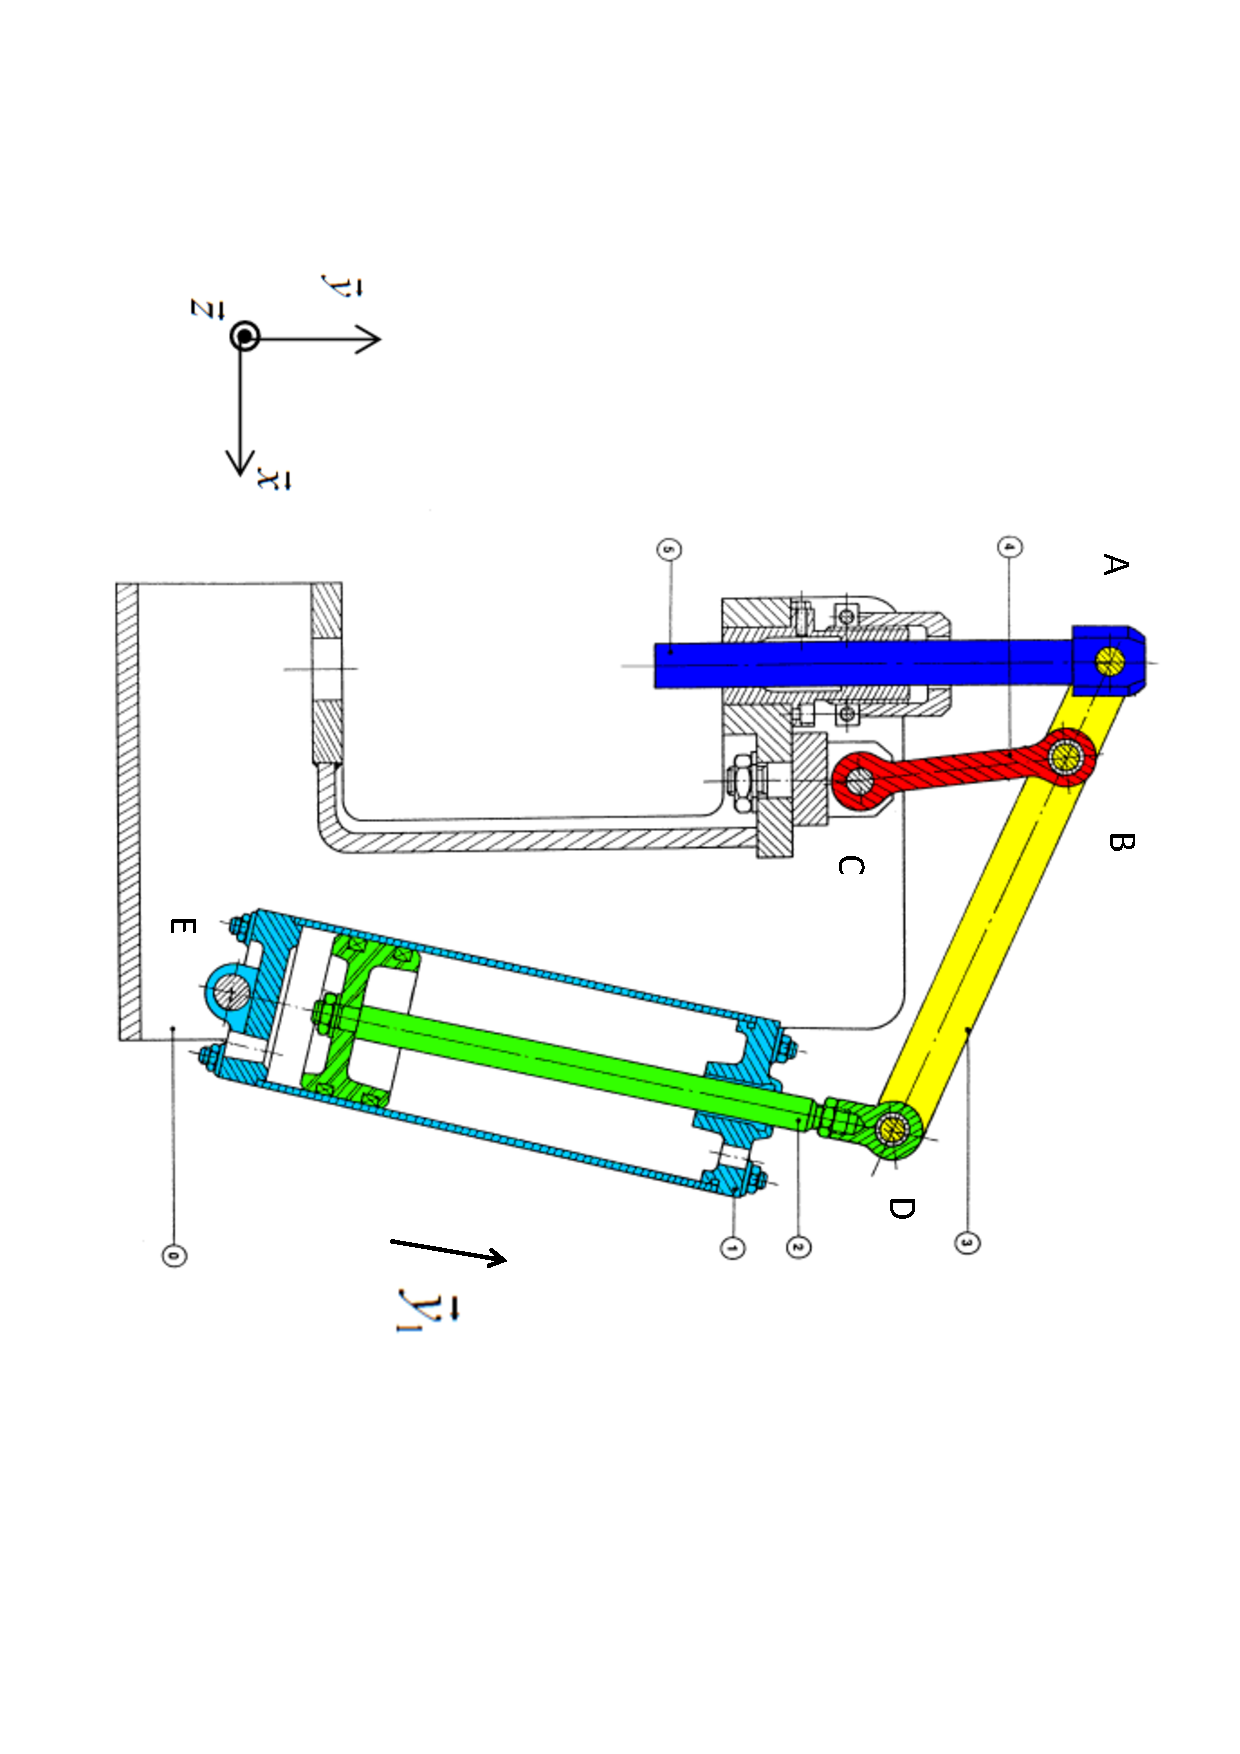
\includegraphics[width=0.95\linewidth]{img/DR05_cor}
\end{center}}

\end{document}
